\section{Autonomous Walking}
\label{sec::42_aw}
The autonomous walking is based upon the performance within the test environment from section \ref{sec::412_pt}. The found parameters are used for comparative reason throughout this section as well. As explained in section \ref{sec::224_ip}, the neural network benefits strongly from an available depth map as input. We will therefore deal with the depth map extraction first.
\subsection{Camera Calibration}
\label{sec::421_cc}
As described in section \ref{sec::224_ip}, in order for the stereo block matching algorithm to work properly (equation \ref{eq::224_sad}), it is required to calibrate the cameras. We shortly verified this in figure \ref{fig::421_no_calib}, where we extracted a depth map from the uncalibrated stereo camera pair.
\begin{figure}[h!]
	\centering
	\subcaptionbox{Left disparity map.}%
	[.4\linewidth]{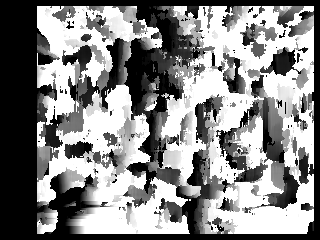
\includegraphics[scale=.3]{chapters/04_experiments/02_autonomous_walking/02_depth_map_parameter_tuning/disp_no_calib.png}}
	\subcaptionbox{Confidence weighted least squares filtered disparity map.}%
	[.4\linewidth]{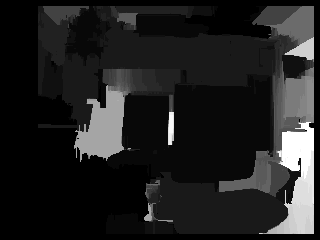
\includegraphics[scale=.3]{chapters/04_experiments/02_autonomous_walking/02_depth_map_parameter_tuning/wls_no_calib.png}}
	\caption{Depth map extraction without calibration. The parameters were set as follows to $N=13$, $D=32$, $\sigma = 1$, and $\lambda=10^4$.}
	\label{fig::421_no_calib}
\end{figure}
For the calibration we chose to use a chess-board calibration pattern, see figure \ref{fig::421_calib}. The used calibration pattern has width of $W=8$, and a height of $H=6$, where each square has a size of $a=22.5\,\text{mm}$ (equation \ref{eq::224_square_size}). We took a total of $N=60$ images of the calibration pattern for varying orientations and translations with respect to the camera, which results in a total of $W\times H\times N = 2880$ points for the calibration. 
\begin{figure}[h!]
	\centering
	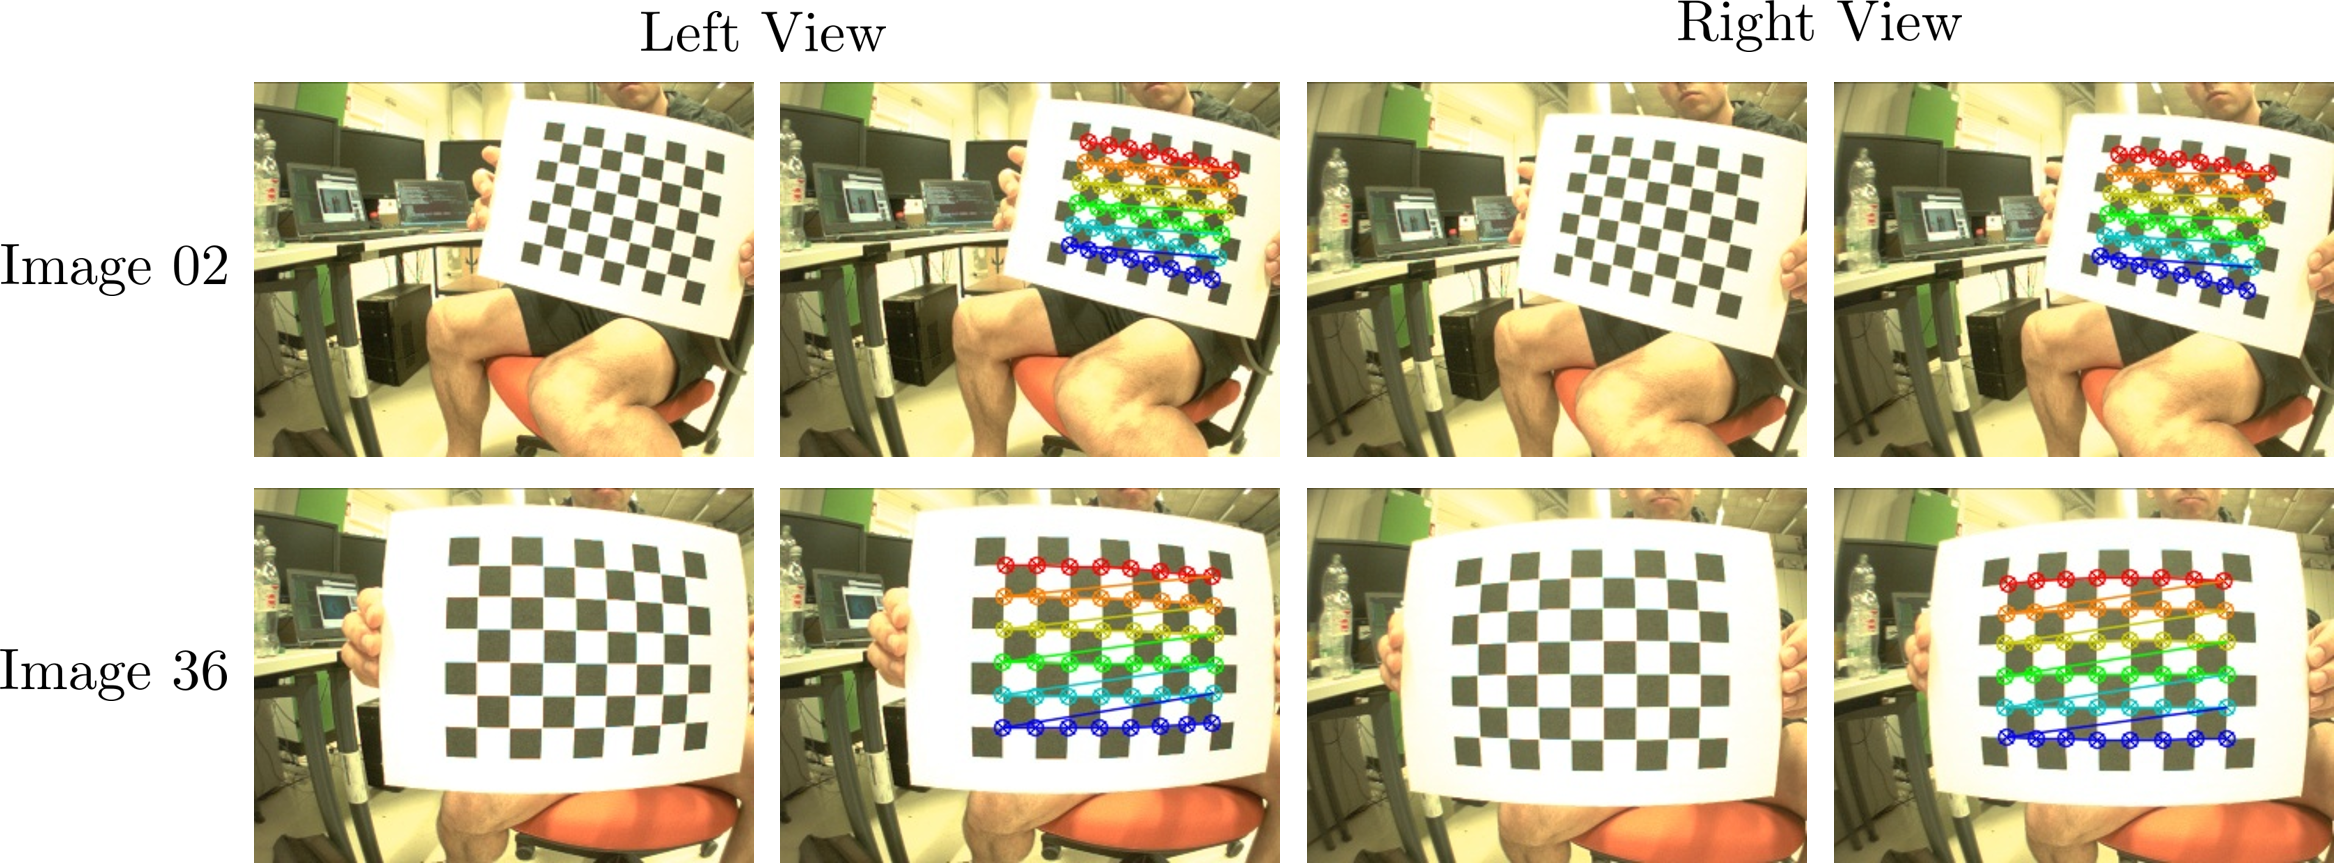
\includegraphics[scale=.28]{chapters/04_experiments/02_autonomous_walking/01_camera_calibration/calib.png}
	\caption{Exemplary left and right camera views of the calibration pattern as acquired during the calibration process. The colorful points indicate the detected corners in the image plane. Refer to figure \ref{fig::224_distortion} for the theory.}
	\label{fig::421_calib}
\end{figure}
As the resulting mean squared re-projection error $\Delta \bar{x} = 1/(WHN)\sum_0^{WHN} \Delta x$ (equation \ref{eq::224_reprojection}), we obtained $\Delta \bar{x}_l = 0.26\, \text{pixel}$, and $\Delta \bar{x}_r = 0.25\,\text{pixel}$, for the left, and the right camera, respectively. According to equations \ref{eq::224_focal_intrinsics}, \ref{eq::224_x_dist}, and \ref{eq::224_y_dist}, we therefore determined the camera's intrinsic parameters as listed in table \ref{tab::421_intrinsics}.
\begin{table}
	\centering
	\caption{Intrinsic parameters of single cameras. These parameters can be found as YAML file on GitHub (\href{https://github.com/mhubii/nmpc_pattern_generator/tree/master/libs/io_module}{\underline{link}}).\label{tab::421_intrinsics}}
	\begin{tabular}{lll}
		Intrinsic Parameter & Left Camera & Right Camera\\
		\hline
		$f_x\,[\text{pixel}/\text{mm}]$ & $\quad2.36\cdot10^2$ & $\quad2.32\cdot10^2$ \\
		$f_y\,[\text{pixel}/\text{mm}]$ & $\quad2.37\cdot10^2$ & $\quad2.32\cdot10^2$ \\
		$c_x\,[\text{pixel}]$ & $\quad1.63\cdot10^2$ & $\quad1.86\cdot10^2$ \\
		$c_y\,[\text{pixel}]$ & $\quad1.11\cdot10^2$ & $\quad1.30\cdot10^2$ \\
		$k_1\,[1/\text{pixel}^2]$ & $-4.54\cdot10^{-1}$ & $-4.58\cdot10^{-1}$ \\
		$k_2\,[1/\text{pixel}^4]$ & $\quad2.90\cdot10^{-1}$  & $\quad3.18\cdot10^{-1}$  \\
		$k_3\,[1/\text{pixel}^6]$ & $-1.21\cdot10^{-1}$ & $-1.48\cdot10^{-1}$ \\
		$p_1\,[1/\text{pixel}]$ & $-2.73\cdot10^{-3}$ & $\quad3.02\cdot10^{-4}$  \\
		$p_2\,[1/\text{pixel}]$ & $\quad2.16\cdot10^{-4}$  & $\quad7.63\cdot10^{-4}$		
	\end{tabular}
\end{table}
Then given the calibration of each single camera, for each camera we computed the rectification transforms $\bm{R}_i$, and the projection matrices $\bm{P}_i$ in the rectified coordinate system, all of which can be found in table \ref{tab::421_extrinsics}.
\begin{table}
	\centering
	\caption{Rectification transforms $\bm{R}_i$, and projection matrices $\bm{P}_i$, for the left, and the right camera, respectively. These parameters can be found as YAML file on GitHub (\href{https://github.com/mhubii/nmpc_pattern_generator/blob/master/libs/io_module/cam_stereo.yaml}{\underline{link}}). \label{tab::421_extrinsics}}
	\begin{tabular}{lll}
		Camera & Extrinsic Parameter & \\ 
		\hline
		&& \\
		\multirow{5}{*}{Left} & $\bm{R}\,[\text{a.u.}]$              & $\begin{pmatrix}
		\quad9.93\cdot10^{-1} & -2.65\cdot10^{-3}     & \quad1.14\cdot10^{-1} \\ 
		\quad5.41\cdot10^{-1} & \quad1.00\cdot10^{0}  & -2.39\cdot10^{-2} \\
		-1.14\cdot10^{-1}     & \quad2.43\cdot10^{-2} & \quad9.93\cdot10^{-1}
		\end{pmatrix}$ \\&&\\
		& $\bm{P}\,[\text{pixel}/\text{mm}]$              & $\begin{pmatrix}
		2.34\cdot10^{2} & 0.00     & 1.88\cdot10^{2} & 0.00\,\text{mm} \\ 
		0.00 & 2.34\cdot10^{2}  & 4.87\cdot10^{1} & 0.00\,\text{mm} \\
		0.00    & 0.00 & 1.00 & 0.00\,\text{mm}
		\end{pmatrix}$ \\
		&&\\
		\multirow{5}{*}{Right} & $\bm{R}\,[\text{a.u.}]$              & $\begin{pmatrix}
		\quad9.95\cdot10^{-1} & -2.30\cdot10^{-2}     & \quad9.93\cdot10^{-2} \\ 
		\quad2.07\cdot10^{-2} & \quad1.00\cdot10^{0}  & \quad2.38\cdot10^{-2} \\
		-9.98\cdot10^{-2}     & -2.16\cdot10^{-2} & \quad9.95\cdot10^{-1}
		\end{pmatrix}$ \\&&\\
		& $\bm{P}\,[\text{pixel}/\text{mm}]$              & $\begin{pmatrix}
		2.34\cdot10^{2} & 0.00     & 1.88\cdot10^{2} & -1.60\cdot10^1\,\text{mm} \\ 
		0.00 & 2.34\cdot10^{2}  & 4.88\cdot10^{1} & 0.00\,\text{mm} \\
		0.00    & 0.00 & 1.00 & 0.00\,\text{mm}
		\end{pmatrix}$ \\
	\end{tabular}
\end{table}
Exemplary rectified images, which rely on the matrices of table \ref{tab::421_extrinsics}, are shown in figure \ref{fig::421_rect} (a). Since there is a slight rotation of the calibration pattern, it is not obvious that the images got rectified well. Therefore, the same images are shown in figure \ref{fig::421_rect} (b), but slightly rotated such that the calibration pattern aligns horizontally. The blue line therein indicates that in contrast to the original image, straight lines now appear straight across both images, which is crucial for the block matching algorithm in the next section - Depth Map Parameter Tuning.
\begin{figure}[h!]
	\centering
	\subcaptionbox{Rectified images.}%
	[.4\linewidth]{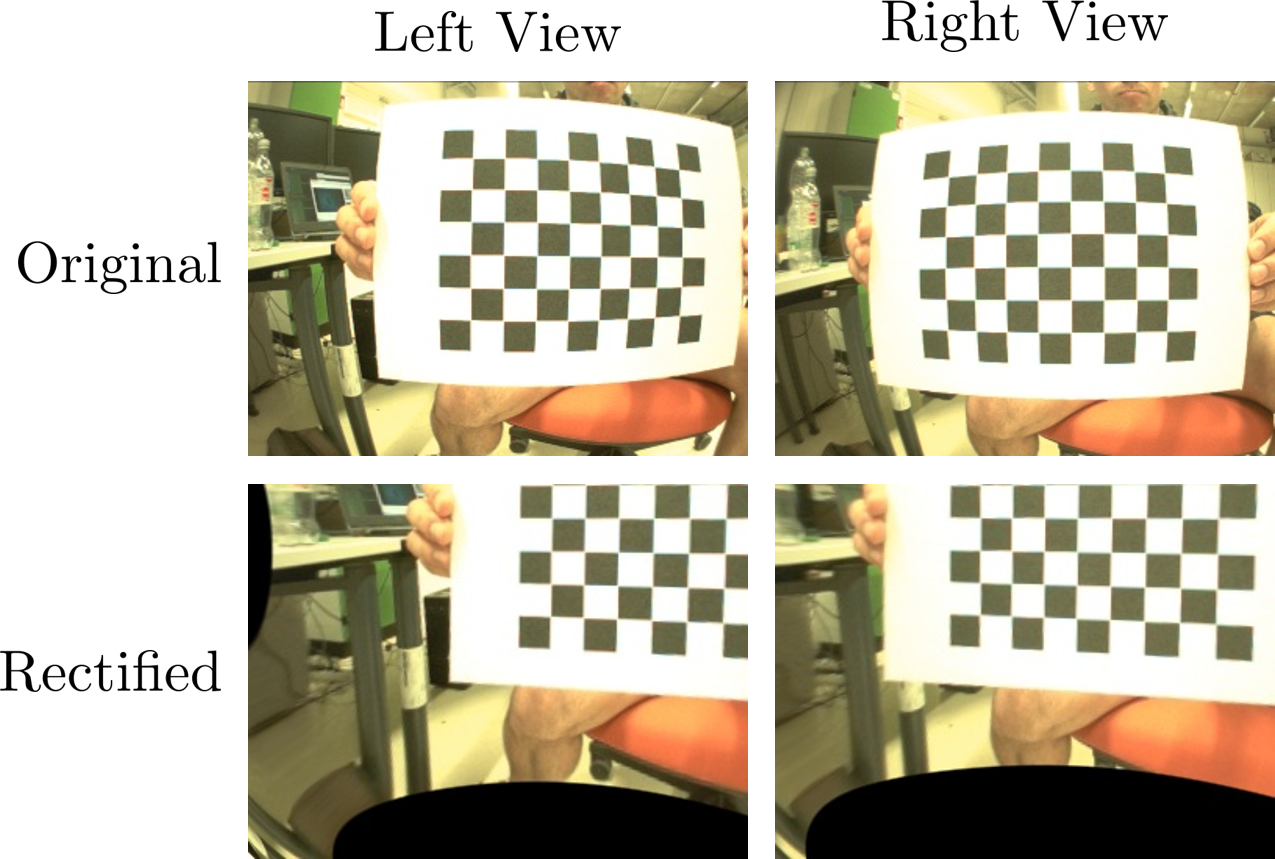
\includegraphics[scale=.25]{chapters/04_experiments/02_autonomous_walking/01_camera_calibration/rect.png}}
	\subcaptionbox{Rotated rectified images.}%
	[.4\linewidth]{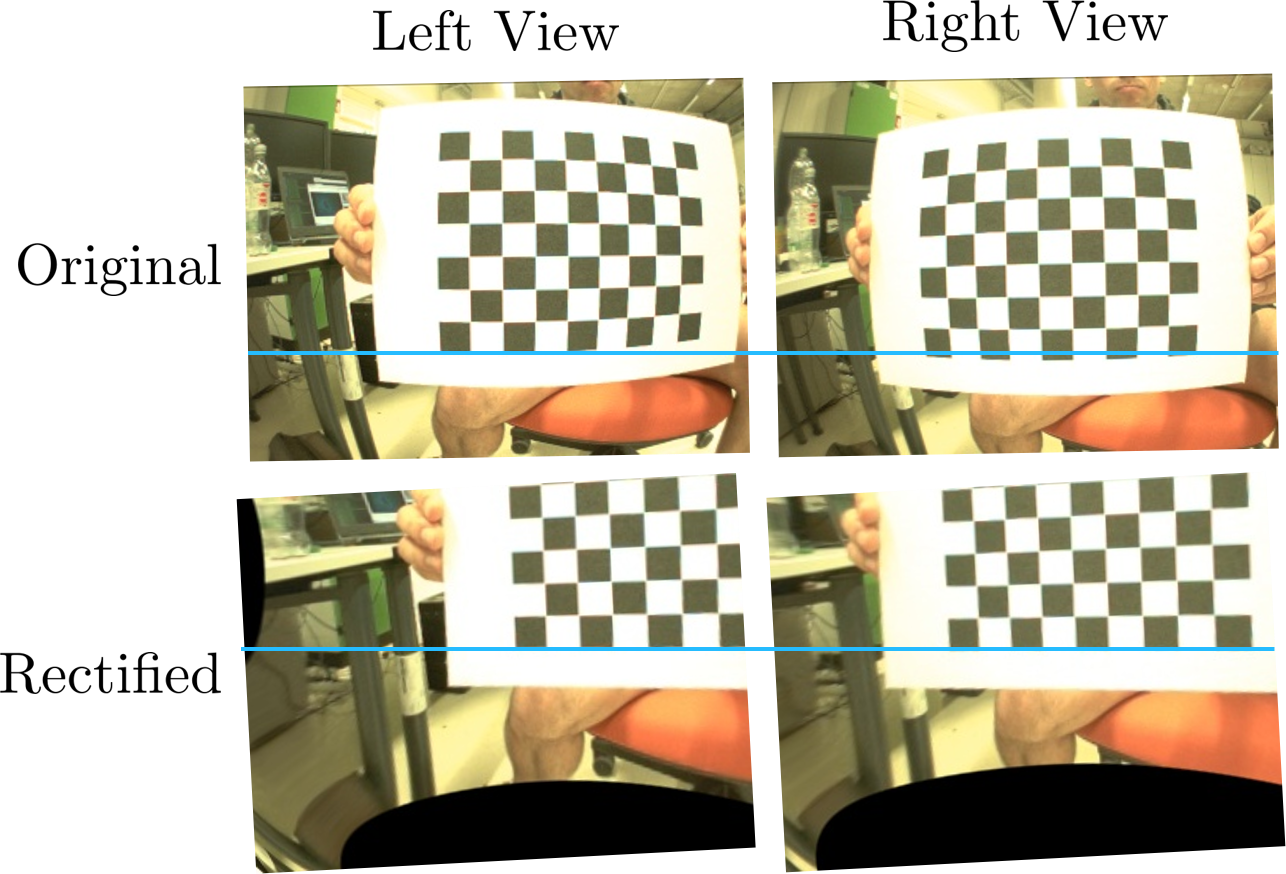
\includegraphics[scale=.25]{chapters/04_experiments/02_autonomous_walking/01_camera_calibration/rect_line.png}}
	\caption{Rectified and original view of the stereo camera. Refer to figure \ref{fig::224_rectified} for the theory.}
	\label{fig::421_rect}
\end{figure}
\subsection{Depth Parameter Tuning}
\label{sec::422_dp}
Within this section, we shortly explore the effects of all tunable parameters on the depth map generation. Therefore, we utilize a simple experimental setup. Within the setup, Heicub points its stereo camera towards three chairs that are located at a distance of $1\,\text{m}$ towards each other, and towards the cameras, so to cover close, medium, and far distances. The consecutive chairs are slightly shifted, in order to enable the simultaneous observation of all of them. The rectified view of the environment is shown in figure \ref{fig::422_wls_rgb}.
\begin{figure}[h!]
	\centering
	\subcaptionbox{Left camera's view.}%
	[.4\linewidth]{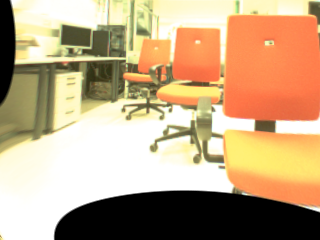
\includegraphics[scale=.3]{chapters/04_experiments/02_autonomous_walking/02_depth_map_parameter_tuning/l_rgb.png}}
	\subcaptionbox{Right camera's view.}%
	[.4\linewidth]{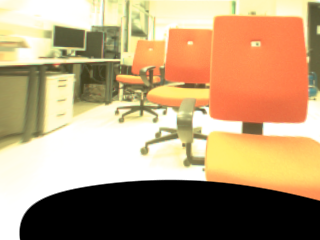
\includegraphics[scale=.3]{chapters/04_experiments/02_autonomous_walking/02_depth_map_parameter_tuning/r_rgb.png}}
	\caption{Heicub's perspective of the scene for the depth map parameter tuning.}
	\label{fig::422_wls_rgb}
\end{figure}
The depth map extraction, which utilizes the rectified images, depends on a stereo block matching algorithm that was explained in section \ref{sec::224_ip}. It mainly depends on the window size and the number of disparities for the sum of absolute difference computation. We evaluate the influence of those two parameters in figure \ref{fig::422_disp} (a) in a grid search fashion. It is apparent that the change in the number of disparities has close to no influence onto the depth map quality, while it removes plenty of useful information from the left hand side of images. The same holds true for the window size, except that it removes some noise from the depth maps.
\begin{figure}[h!]
	\centering
	\subcaptionbox{Left disparity. Please refer to figure \ref{fig::224_left_disparity_map} and equation \ref{eq::224_sad} for the theory.}%
	[.45\linewidth]{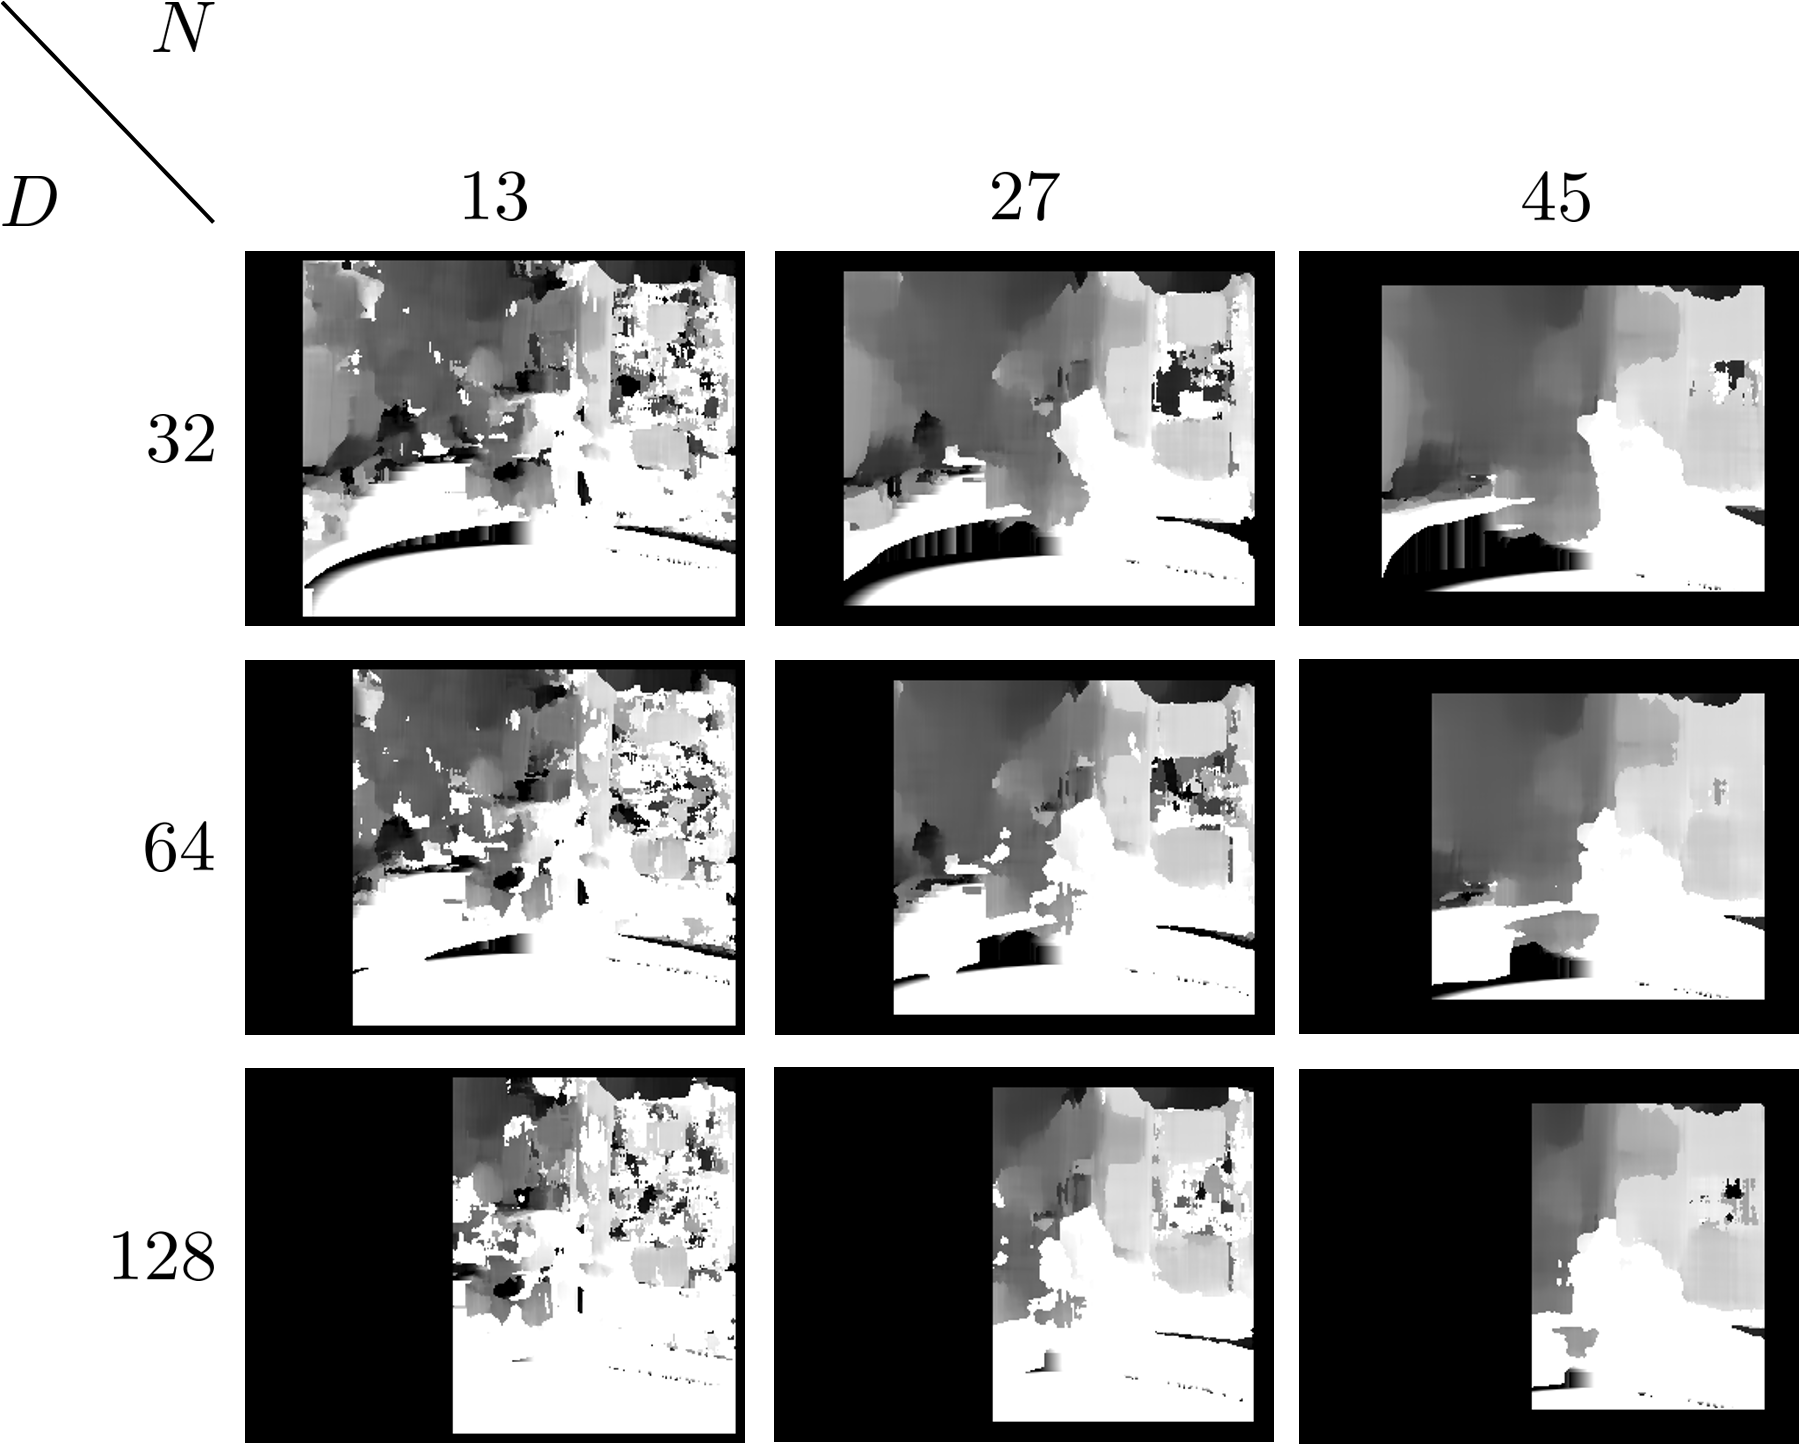
\includegraphics[scale=.2]{chapters/04_experiments/02_autonomous_walking/02_depth_map_parameter_tuning/disp_sad.png}}
	\subcaptionbox{Confidence weighted least squares disparity map. Please refer to figure \ref{fig::224_weighted_least_squares_disparity} and equation \ref{eq::224_wls_final} for the theory.}%
	[.45\linewidth]{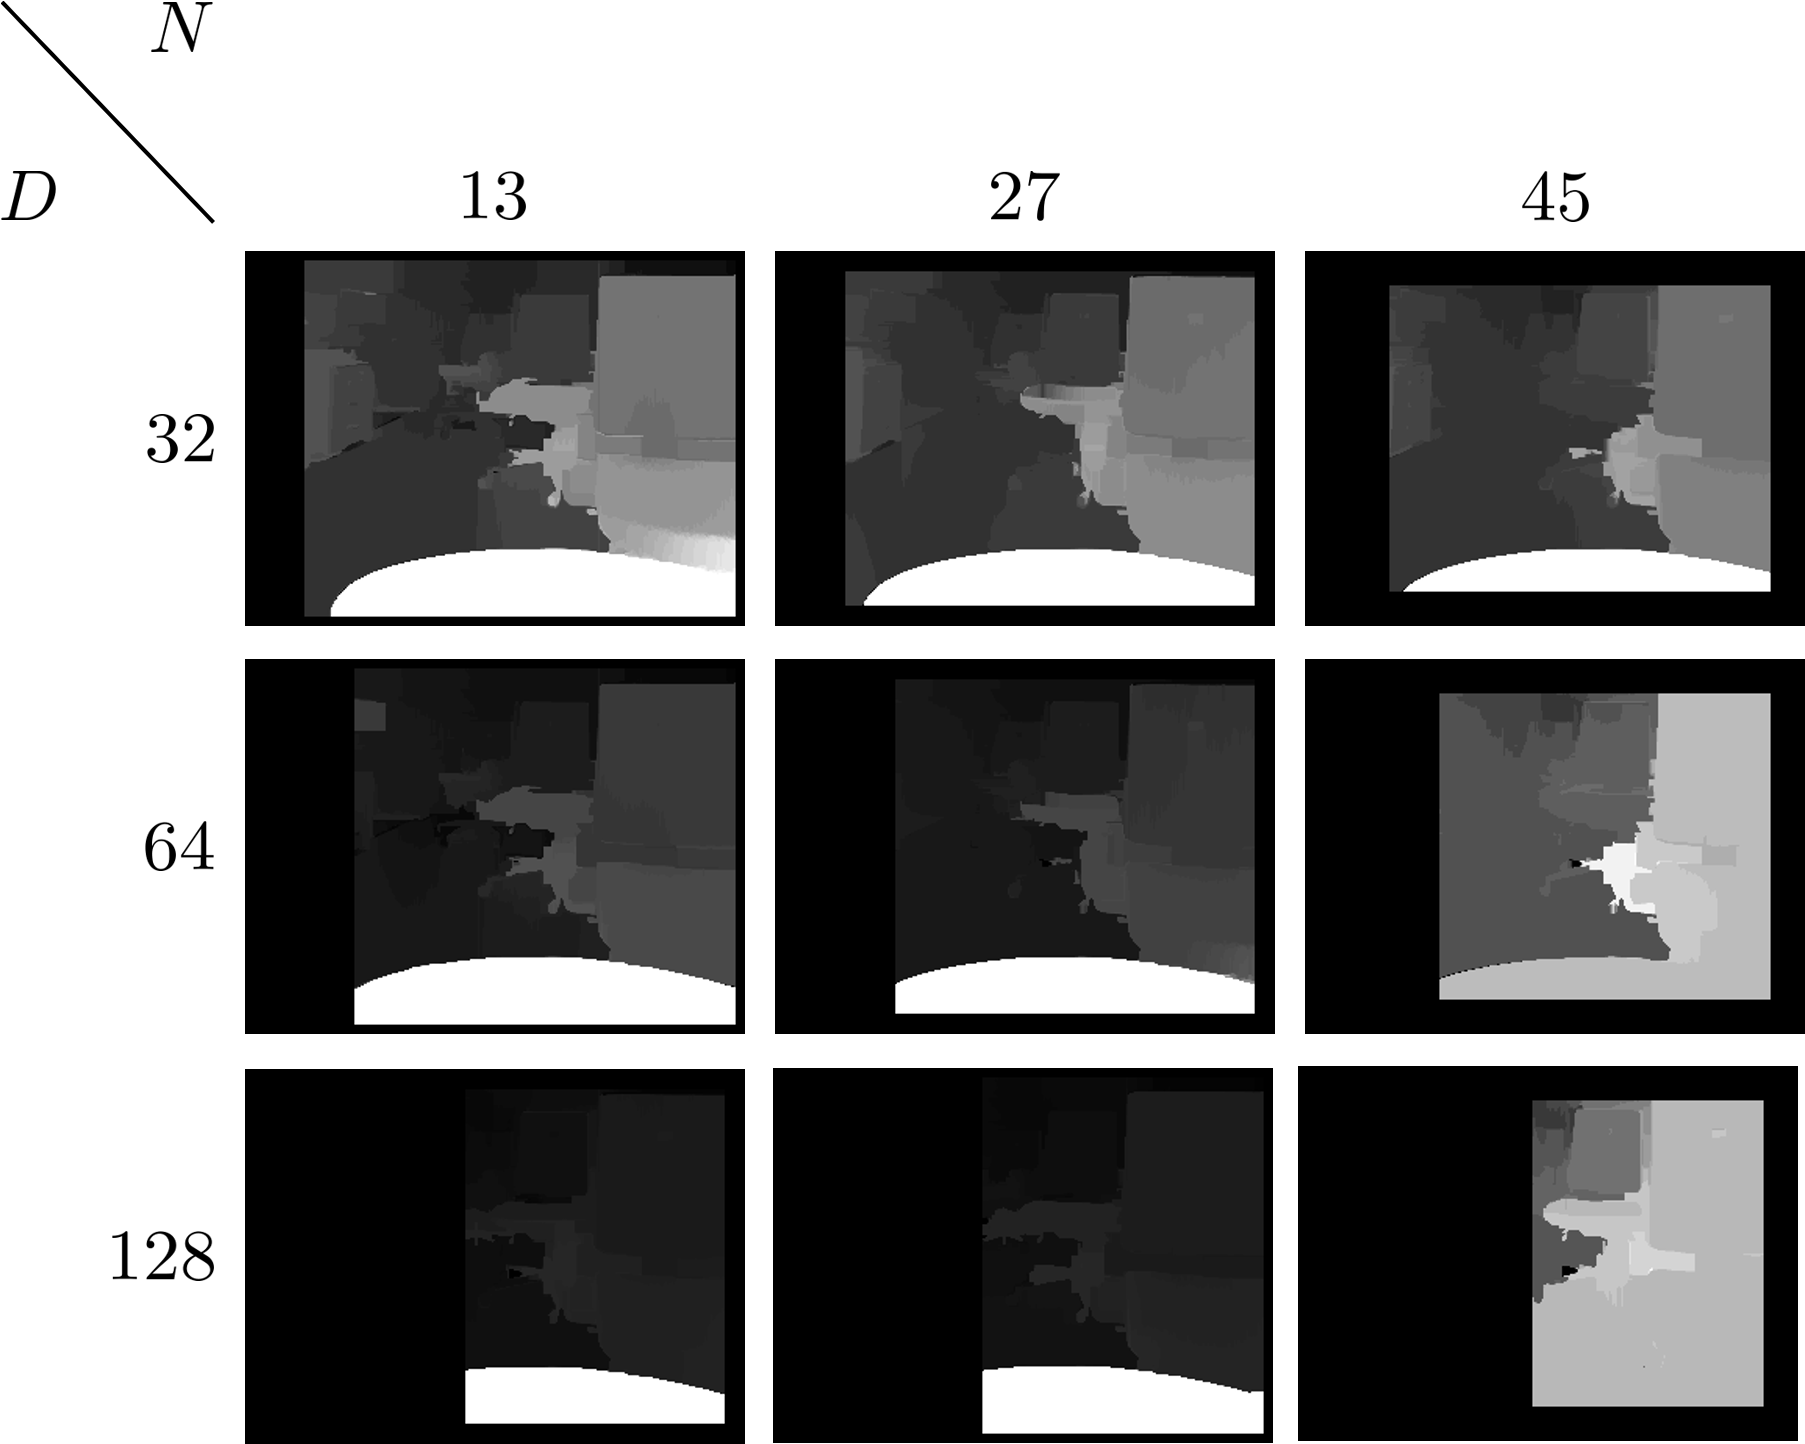
\includegraphics[scale=.2]{chapters/04_experiments/02_autonomous_walking/02_depth_map_parameter_tuning/disp_sad_wls.png}}
	\caption{Left disparity map and confidence weighted least squares disparity for changing SAD window sizes $N$ and number of disparities $D$.}
	\label{fig::422_disp}
\end{figure}
In combination with the confidence weighted least squares filtering, we can observe that most of the noise is already removed (figure \ref{fig::422_disp} (b)), for which it is more import to keep the information close to the images' borders. We therefore chose to set the number of disparities $D=32$, and the windows size $N=13$ in the following. Within these depth maps, the global energy weighting $\lambda$ was set to $10^4$, and the local bilateral filter decay $\sigma$ to $1$, since we observed the best performance for them. The influence of those two parameters is visualized in figure \ref{fig::422_sigma_lambda}. We can see that, in good accordance with the theory, $\sigma$ contributes to the smoothing of the depth map, and that $\lambda$ enforces a change in depth across edges within the RGB images.
\begin{figure}[h!]
	\centering
	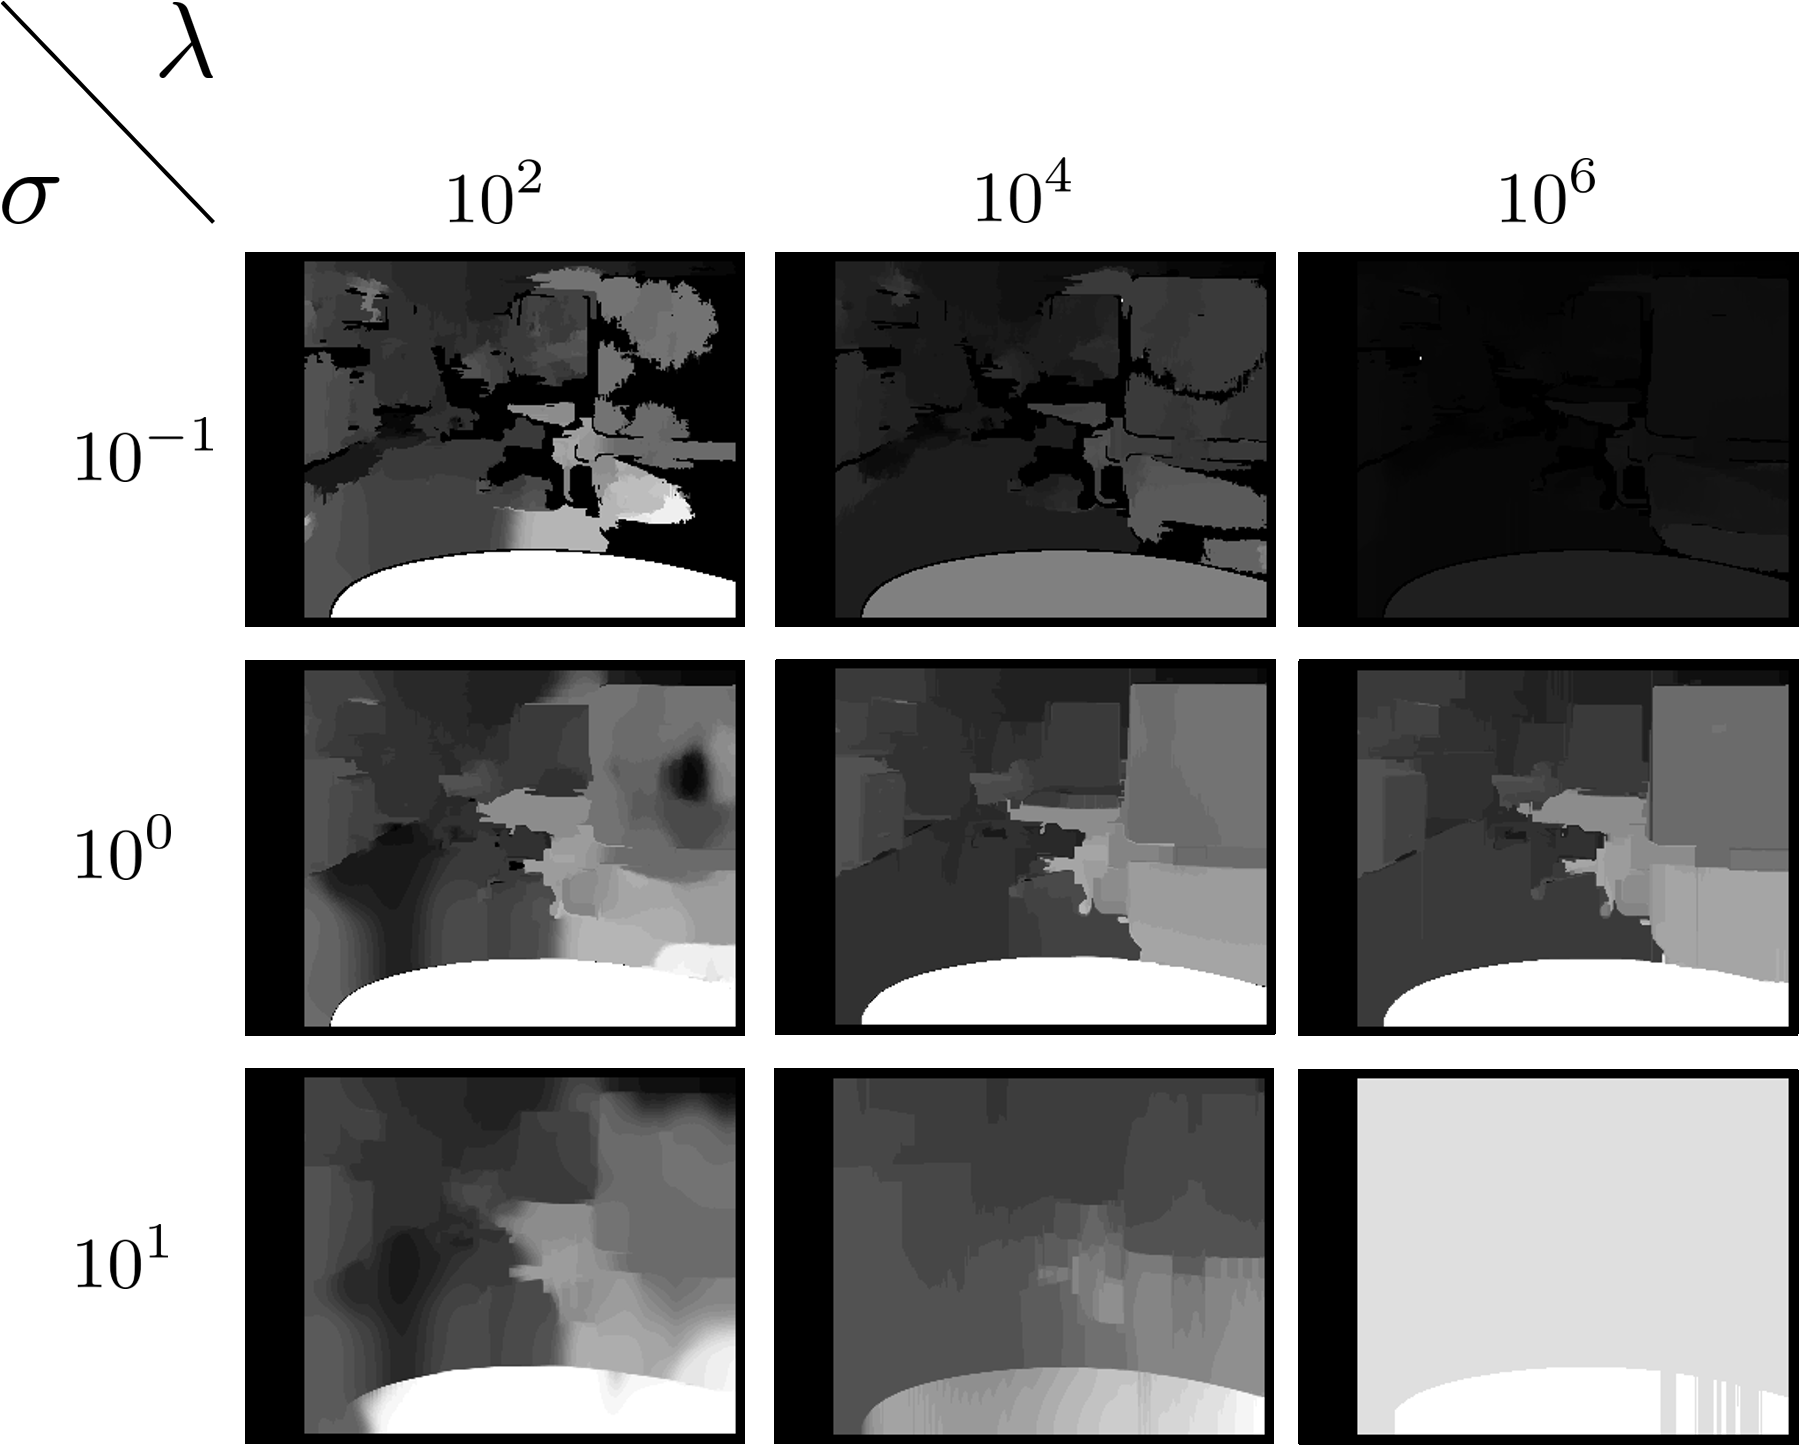
\includegraphics[scale=.2]{chapters/04_experiments/02_autonomous_walking/02_depth_map_parameter_tuning/sigma_lambda.png}
	\caption{Confidence weighted least squares disparity for changing energy weightings $\sigma$ and $\lambda$. Please refer to equations \ref{eq::224_weight} and \ref{eq::224_energy_function} for the theory.}
	\label{fig::422_sigma_lambda}
\end{figure}
\subsection{Data Acquisition and Training}
\label{sec::423_da}
As already pointed out, the task we wanted our neural network to solve was to find a fire extinguisher within a room and then to move towards it. For us to apply behavioral cloning to the task, it was necessary to act according to this policy first, and then to train a neural network on the acquired data. For the data, it is essential to sample homogeneously over the task's distribution. We therefore recorded velocity commands and the corresponding images for 66 distinct epochs. Each of the epochs was designed to reflect different scenarios, among them obstacle avoidance, interaction with humans, walking towards the fire extinguisher, and searching for the fire extinguisher when it was not possible to directly see it. As a result of the observations that we gained from the user controlled walking in section \ref{sec::41_uc}, we restricted the user's policy to only use linear velocities along the x-axis, and angular velocities about the z-axis, since linear velocities along the y-axis revealed to pose an inefficient way of moving the robot. Exemplary samples of the recorded dataset are presented in figure \ref{fig::423_dataset}.
\begin{figure}[h!]
	\centering
	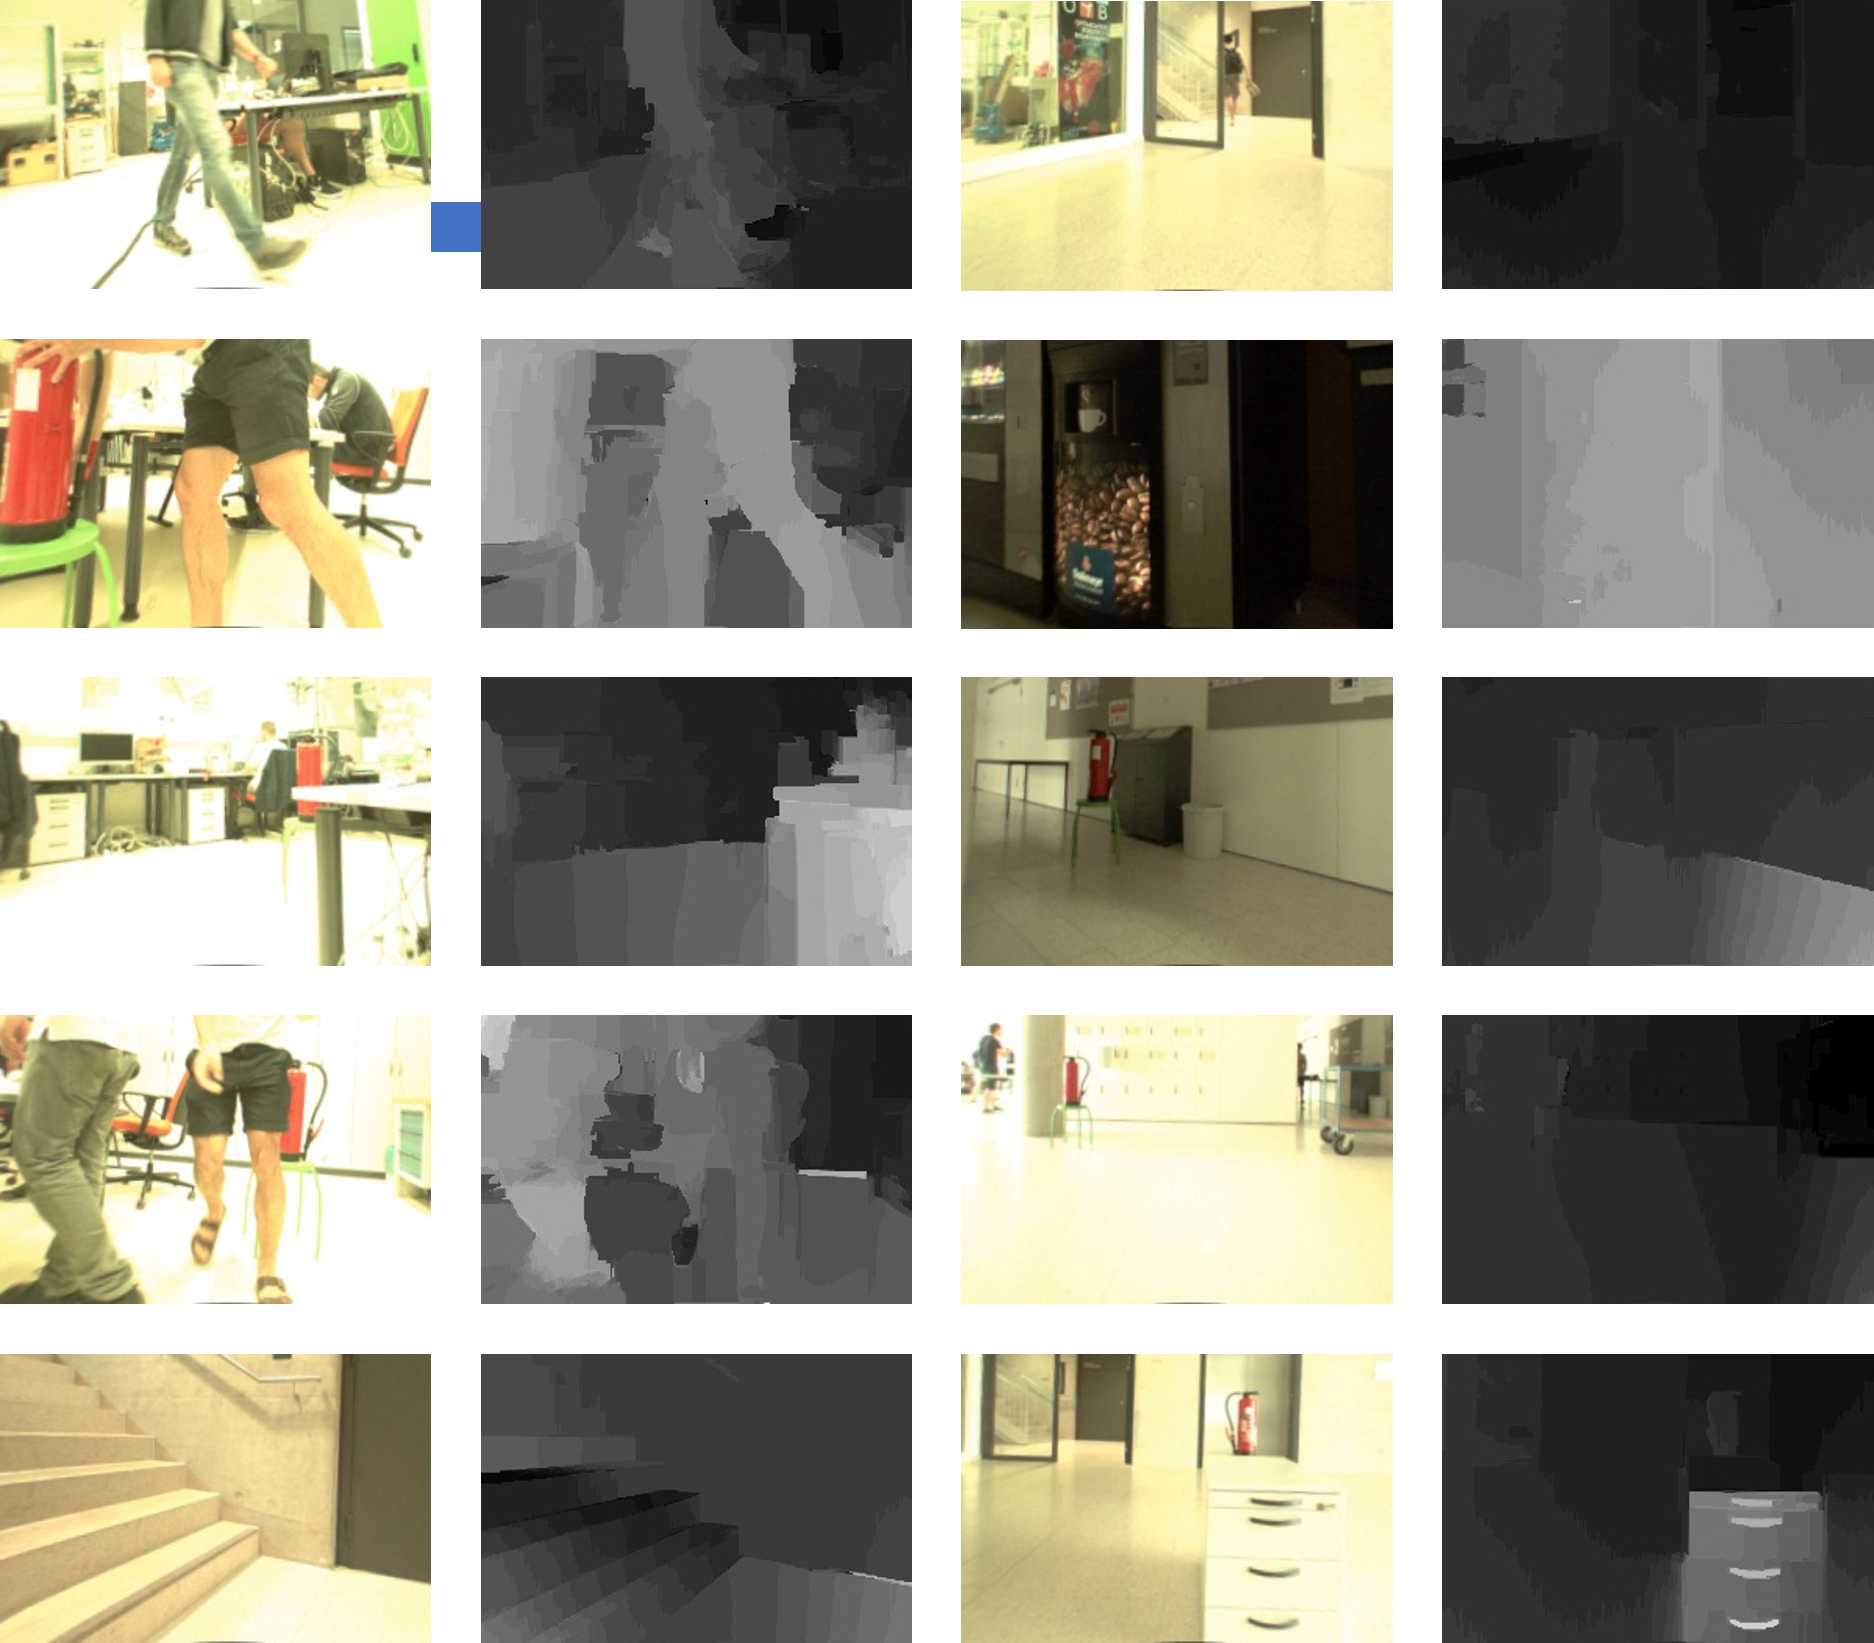
\includegraphics[scale=.4]{chapters/04_experiments/02_autonomous_walking/dataset_diversity.png}
	\caption{Samples of the recorded dataset. The dataset shows a very diverse number of situation for the neural network to learn from.}
	\label{fig::423_dataset}
\end{figure}
It contains 134401 samples in total, which were recorded at a rate of 5 frames per second, and therefore they account for roughly 7.5 hours of data. For each sample, we stored the left camera's RGB view, as well as the confidence weighted least squares disparity map. This lead to a total of 268802 recorded images at a resolution of $240\times320$ pixels, which together make up for $4.7\,\text{GB}$ of data. As a preprocessing step, we cropped regions of the recorded images that do not contain useful information. These regions are firstly caused by deformations that are introduced at the rectification step, as can for example be seen in figure \ref{fig::422_wls_rgb}, and secondly by the depth map's extraction, which results in unknown regions at the image's boarders (figure \ref{fig::422_disp}). The exemplary samples from the dataset (figure \ref{fig::423_dataset}), are already preprocessed, and we can observe how only useful information is kept, in order not to confuse the neural network. To reduce the required amount of GPU memory, we further downscaled the preprocessed images to a size of $60\times80$ pixels, a size at which most of the information is still being kept, and stacked the RBD images with the confidence weighted least squares disparity map to obtain RBGD images. For the training of the neural network, we split the acquired dataset into a training, and a validation set. The training set held a randomly sampled fraction of $90\%$ of all recorded images, while the validation split held the other $10\%$. We only trained the neural network on the training set, and stored the weights that performed best on the validation split, in order to avoid overfitting. Since it has shown very good convergence on our dataset, we chose to use a UNet \cite{ronneberger2015u} as the network architecture, which can be seen in figure \ref{fig::423_unet}.
\begin{figure}[h!]
	\centering
	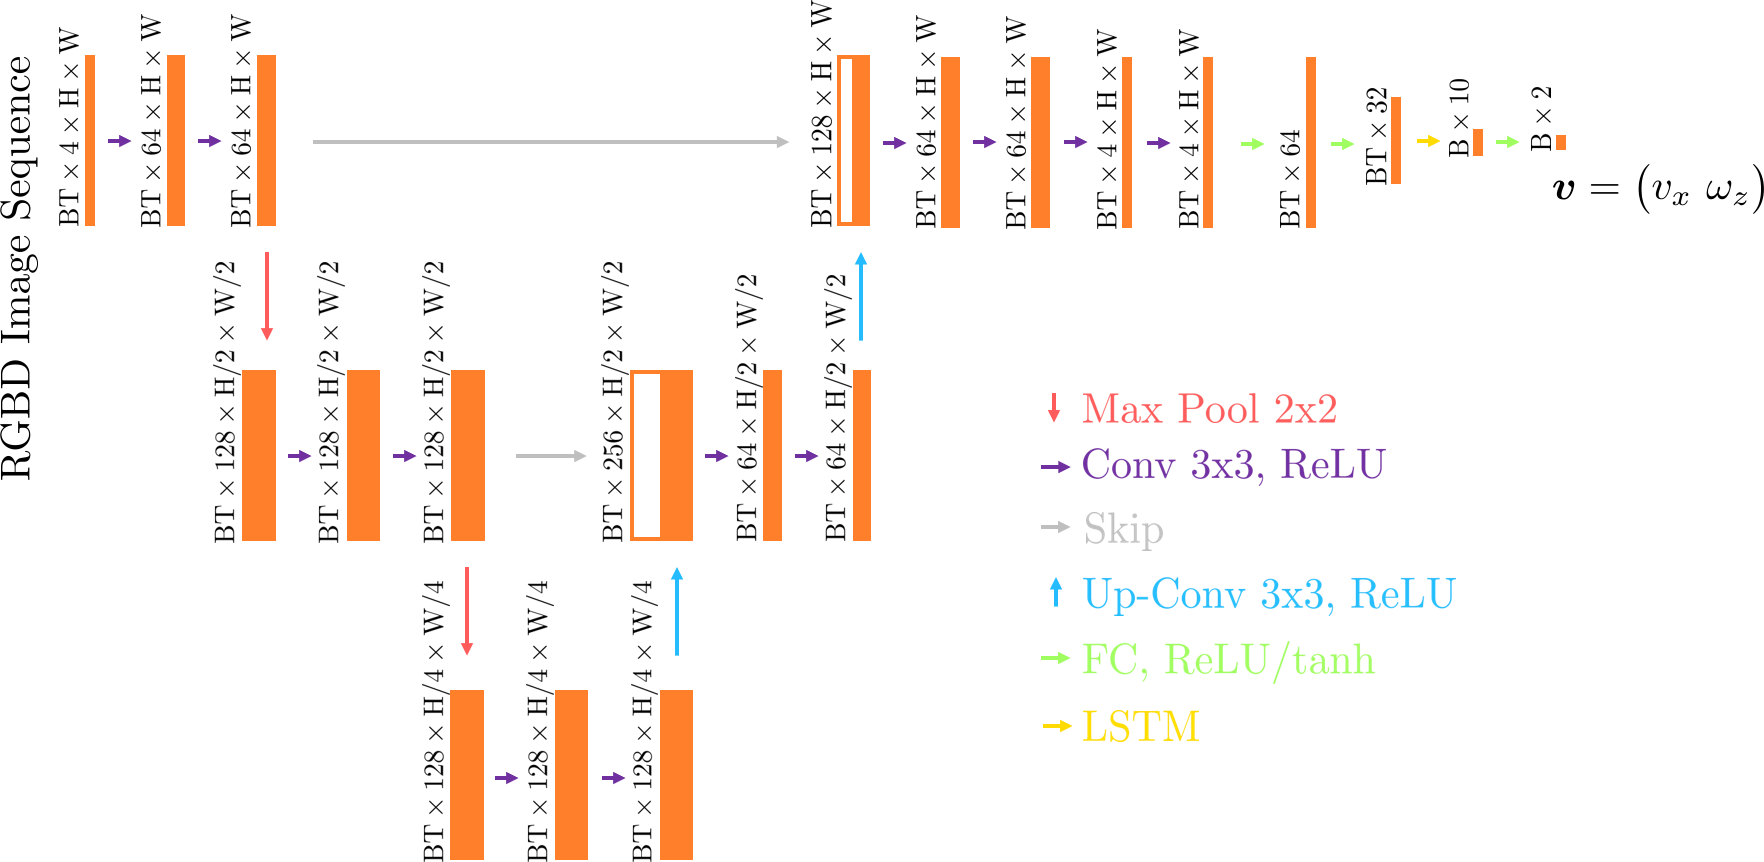
\includegraphics[scale=.5]{chapters/04_experiments/02_autonomous_walking/unet.png}
	\caption{UNet-LSTM network architecture.}
	\label{fig::423_unet}
\end{figure}
The UNet promotes image abstraction capabilities of an auto-encoder that is caused by its bottleneck design, and furthermore shows faster convergence due to its residual connections, which allow the gradient flow to reach deeper layers earlier. Each image that is being forwarded, goes through a number of convolutional layers with rectifying linear unit activation functions, and is subsequently downscaled by max-pooling operations. We repeated this process for two times. Once the most downscaled layer is reached, the weights are being upscaled by simple interpolations again, which simply results in the same resolution that the layers had during the downscaling process. The skip connections then concatenate the shallow with the deep layers to a new layer at each scale, which is then being forwarded further through a number of convolutional layers with rectifying linear units. The nature of the robot's motion, which inherently causes the cameras to periodically move from the left to the right, required us to equip the network architecture by a temporal understanding. We therefore extended the UNet architecture to a novel UNet-LSTM structure. The developed architecture takes up a sequence of consecutive RGBD images, and forwards them through the UNet until it reaches a fully connected regression layer that shall output velocity values in the end. Each image therein creates a signal, from which the LSTM is supposed to only keep the most relevant information. This design helped the network to understand that a fire extinguisher to the left of the image may only be caused by the cameras that are temporally displaced to the right. The last fully connected layer then returns what we use for the loss function, and therefore a velocity. In contrast to the preceding layers, the last fully connected layer uses a hyperbolic tangent function, which restricts the output to a range of $[-1,1]$, which is then being scaled by the velocity that the pattern generator maximally allows. The architecture can be found at the provided \href{https://github.com/mhubii/nmpc_pattern_generator/blob/master/libs/learning/python/unet_model.py}{\underline{link}}. Due to memory limitations, we trained the network on a sequence length of 5 RGBD images, and a batch size of 32. For the loss, we chose a mean squared error with respect to the most recent velocity command. We used the Adam optimization \cite{kingma2014adam} at a learning rate of  $0.001$, and trained for 100 epochs on a Nvidia GTX 1080 with $8\,\text{GB}$ RAM, to which we were granted access to. This took us around 48 hours. The loss history is shown in figure \ref{fig::423_loss}, which reveals a good convergence after around 40 epochs.
\begin{figure}[h!]
	\centering
	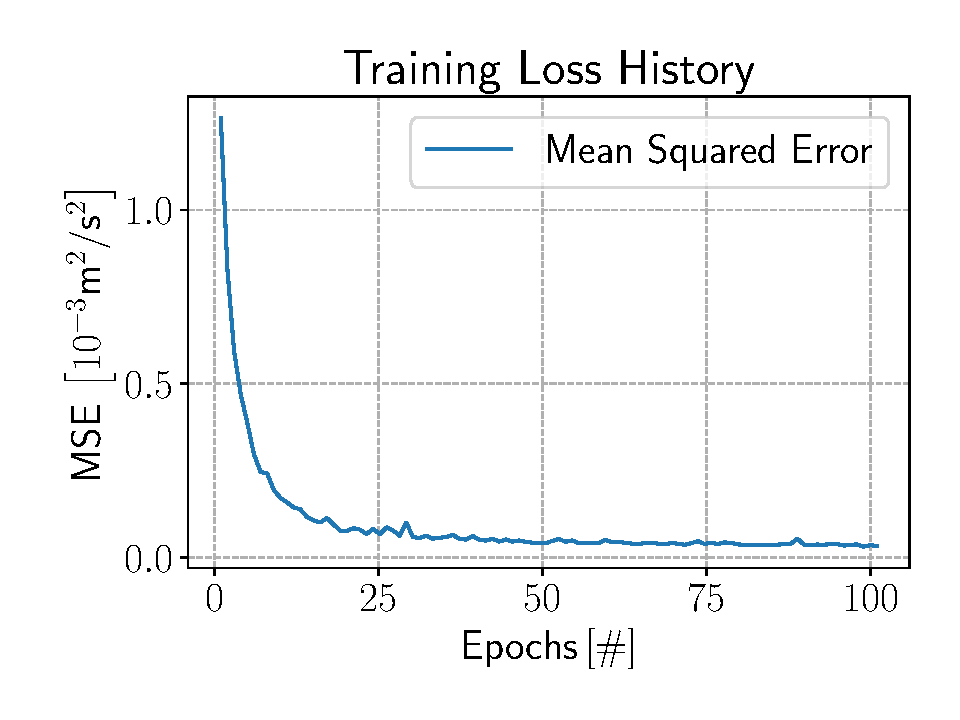
\includegraphics[scale=.4]{chapters/04_experiments/02_autonomous_walking/05_07_19_loss_history.pdf}
	\caption{Mean squared error training loss history of the UNet on the validation split of the dataset, shown in figure \ref{fig::423_unet}.}
	\label{fig::423_loss}
\end{figure}
After training, we generated velocity histograms, as we already did in section \ref{sec::41_uc}, but this time over the whole validation split for both, the ground truth and the predicted behavior, as shown in figure \ref{fig::423_training_dist}. To generate the predictions on the validation split took $4\,\text{ms}$ with a GeForce GTX 1050 for each of the 13341 images on average.
\begin{figure}[h!]
	\centering
	\subcaptionbox{Ground truth velocity commands.}%
	[.45\linewidth]{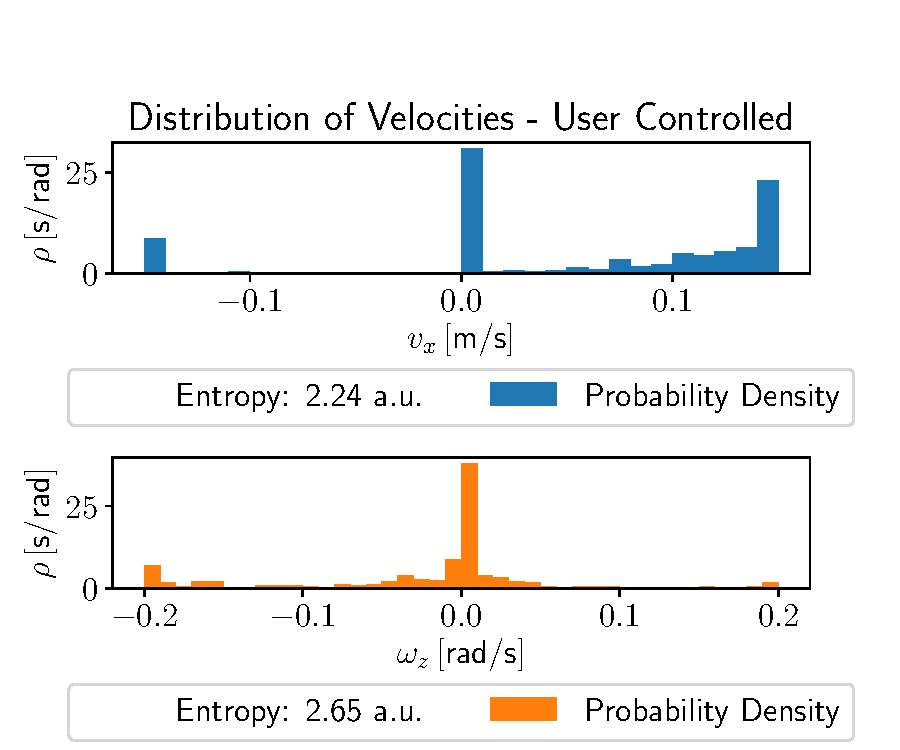
\includegraphics[scale=.45]{chapters/04_experiments/02_autonomous_walking/user_entropy.pdf}}
	\subcaptionbox{Predicted velocity commands.}%
	[.45\linewidth]{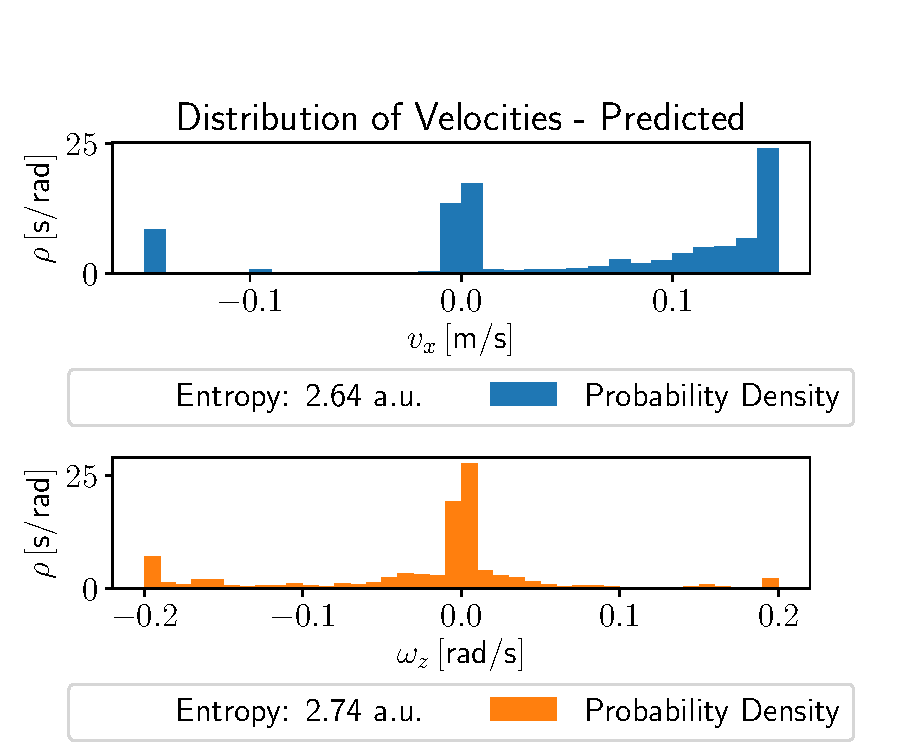
\includegraphics[scale=.45]{chapters/04_experiments/02_autonomous_walking/predicted_entropy_kldivx_0_33_kldivz_0_06_imgs_13441_duration_4_ms.pdf}}
	\caption{Normalized velocity histograms over the validation split. The ground truth (a), and the predicted velocity commands (b), appear to be very similar., which indicates a successful training.}
	\label{fig::423_training_dist}
\end{figure}
By pure sight, it can already be seen that the network performs well on the validation split, and the Kullback-Leibler divergence $D_\text{KL}$, which measures the distance of probability distributions, enforces this observation further. The Kullback-Leibler divergence for two discrete probability distributions $p(v)$ and $q(v)$, is computed as follows
\begin{align}
	D_\text{KL} = \sum_{v\in \bm{V}}p(v)\log\frac{p(v)}{q(v)},
\end{align}
where for our case, $p(v)$ is the ground truth velocity distribution, and $q(v)$ is the predicted velocity distribution. For the distribution of linear velocities along the x-axis $v_x$, we computed the Kullback-Leibler divergence to be $D^x_\text{KL}=0.33\,\text{a.u.}$, and for the angular velocity about the z-axis $\omega_z$, we obtained $D^z_\text{KL}=0.06\,\text{a.u.}$. Now the beauty within the task at hand lies in the fact that we were not solely dependent on a validation split for performance evaluations, but instead that we simply could run Heicub in a previously unseen test environment. It is the same test environment, which we already introduced in section \ref{sec::41_uc}, and we will evaluate the trained neural network's behavior within it in the next section - Perfomance in Test Environment.
\subsection{Performance in Test Environment}
\label{sec::424_pt}
For the performance benchmarking, we relied on the well defined experimental setup from section \ref{sec::41_uc}. Once more the tasks were to move straight towards a fire extinguisher, to turn and to move towards it, to avoid an obstacle on the way, and to find the fire extinguisher. In order to ensure reproducibility, we let Heicub solve each of these tasks twice, as we did for the user controlled case. The setup is shown in figure \ref{fig::424_aw_gif_basic}, which shows Heicub's movement over the course of each task along with its sight of the scene.
\begin{figure}[h!]
	\centering
	\subcaptionbox{Straight walk - \href{https://drive.google.com/file/d/1X-RQ9yVLJ9McgeXVoDQhI1uvMJA5o08y/view?usp=sharing}{\underline{link}}.}%
	[.4\linewidth]{\animategraphics[height=1.2in,loop,autoplay]{20}{chapters/04_experiments/02_autonomous_walking/straight_walk_01/frame-}{001}{033}}
	\subcaptionbox{Curved walk - \href{https://drive.google.com/file/d/1TpT7PUw8cWaUvy1toccXsNO_lQQFlFIS/view?usp=sharing}{\underline{link}}.}%
	[.4\linewidth]{\animategraphics[height=1.2in,loop,autoplay]{20}{chapters/04_experiments/02_autonomous_walking/curved_walk_02/frame-}{001}{039}}
	\subcaptionbox{Obstacle avoidance - \href{https://drive.google.com/file/d/1DlO8Rd6AiBPrHKbTIgI12d2ySaTvMJ3S/view?usp=sharing}{\underline{link}}.}%
	[.4\linewidth]{\animategraphics[height=1.2in,loop,autoplay]{20}{chapters/04_experiments/02_autonomous_walking/obstacle_walk_02/frame-}{001}{017}}
	\subcaptionbox{Environment scanning - \href{https://drive.google.com/file/d/1QmtltYTwoXMzHoUA8knA2FEpMsaud0QD/view?usp=sharing}{\underline{link}}.}%
	[.4\linewidth]{\animategraphics[height=1.2in,loop,autoplay]{20}{chapters/04_experiments/02_autonomous_walking/out_of_sight_walk_01/frame-}{001}{075}}
	\caption{Heicub's behavior in the test environment for the benchmarking tasks. The robot within these trials was controlled by the Unet model, shown in figure \ref{fig::423_unet}.}
	\label{fig::424_aw_gif_basic}
\end{figure} 
While Heicub did manage to solve the straight walk, the curved walk, and the environment scanning, it had trouble to go towards the fire extinguisher, once it avoided the obstacle. Again, we tracked the zero moment point from the pattern generator, as well as the true zero moment point from the force torque readouts. The results of these measurements are shown in figures \ref{fig::424_aw_basic_straight} - \ref{fig::424_aw_basic_sight}. It can clearly be seen that the neural network's behavior for within the test environment is much noisier than it was for the validation split in figure \ref{fig::423_training_dist}. This especially holds true for the angular velocity distributions. 
\begin{figure}[h!]
	\subcaptionbox{Dynamic balance.}%
	[.5\linewidth]{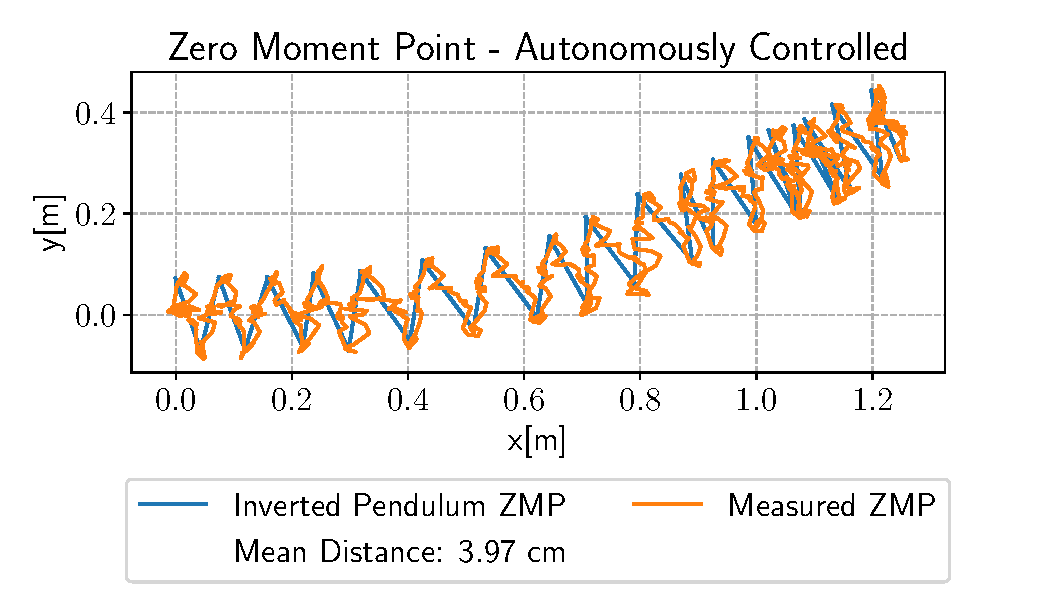
\includegraphics[scale=.45]{chapters/04_experiments/02_autonomous_walking/straight_walk_01_zmp.pdf}}
	\subcaptionbox{Behavior.}%
	[.5\linewidth]{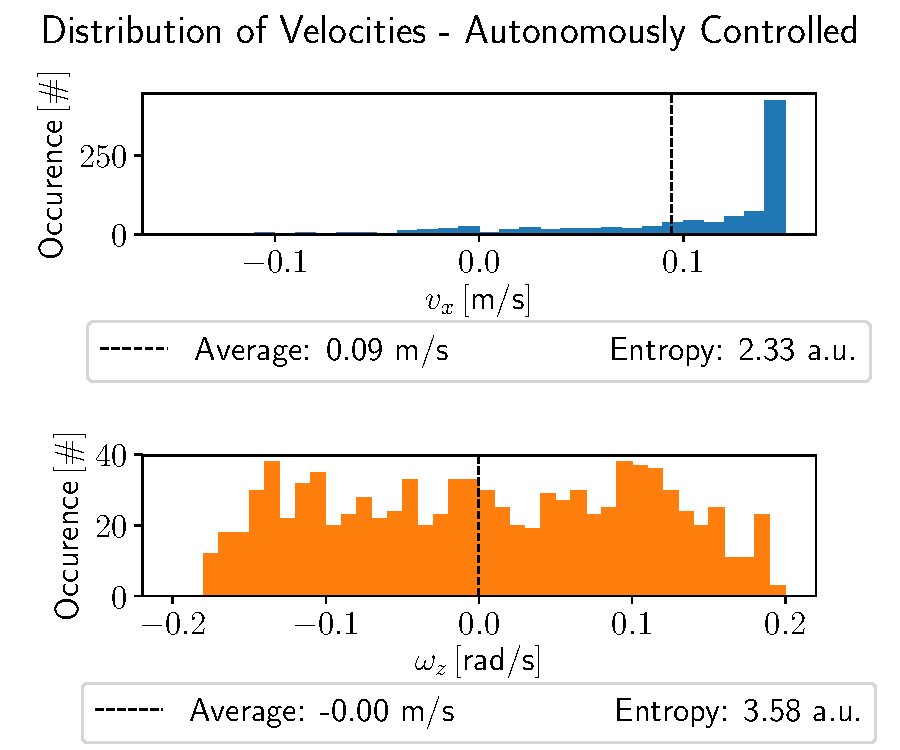
\includegraphics[scale=.45]{chapters/04_experiments/02_autonomous_walking/straight_walk_01_entropy.pdf}}
	\caption{Autonomously controlled straight walk. The robot started to the plot's left hand side (a), and then moved straight towards the fire extinguisher until it stopped infront of it.}
\label{fig::424_aw_basic_straight}
\end{figure} 
\begin{figure}[h!]
	\subcaptionbox{Dynamic balance.}%
	[.5\linewidth]{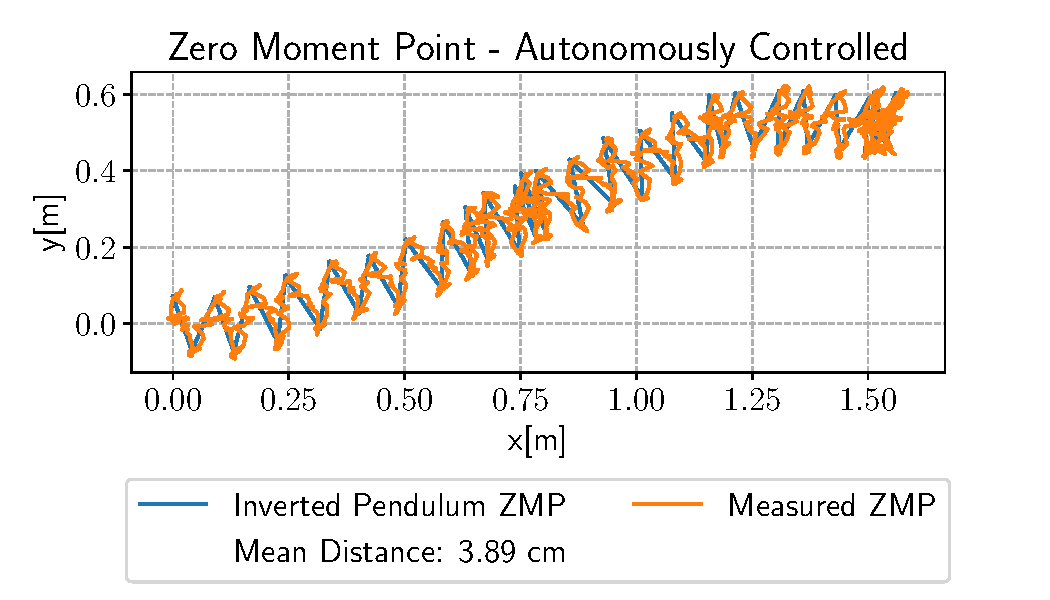
\includegraphics[scale=.45]{chapters/04_experiments/02_autonomous_walking/curved_walk_01_zmp.pdf}}
	\subcaptionbox{Behavior.}%
	[.5\linewidth]{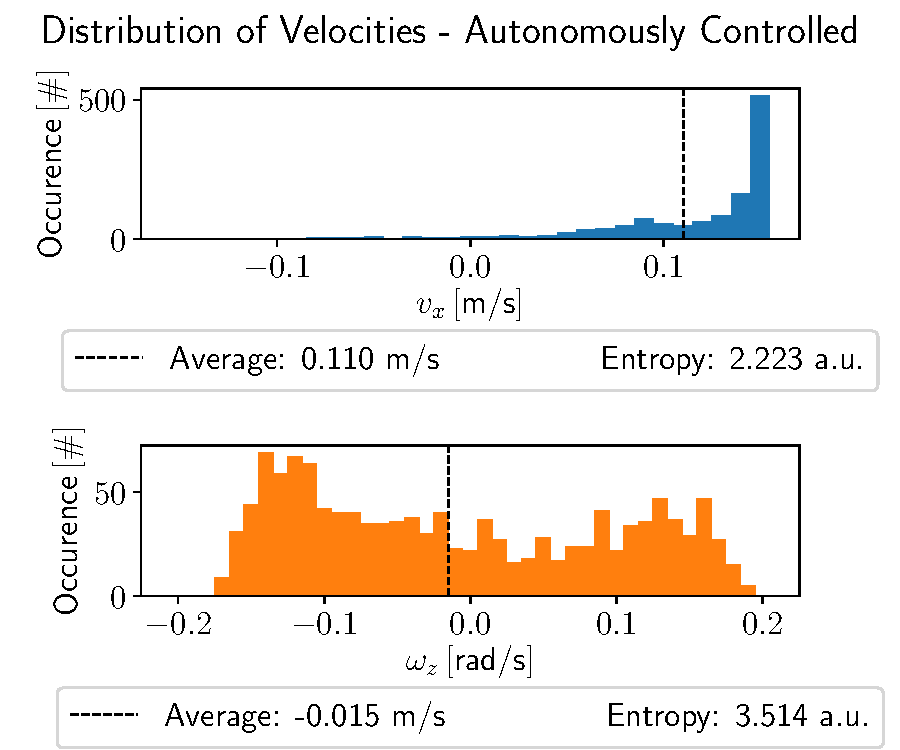
\includegraphics[scale=.45]{chapters/04_experiments/02_autonomous_walking/curved_walk_01_entropy.pdf}}
	\caption{Autonomously controlled curved walk. The robot started to the plot's left hand side (a), and moved on a curved line towards the fire extinguisher, which was located to its left.}
\label{fig::424_aw_basic_curved}
\end{figure} 
\begin{figure}[h!]
	\subcaptionbox{Dynamic balance.}%
	[.5\linewidth]{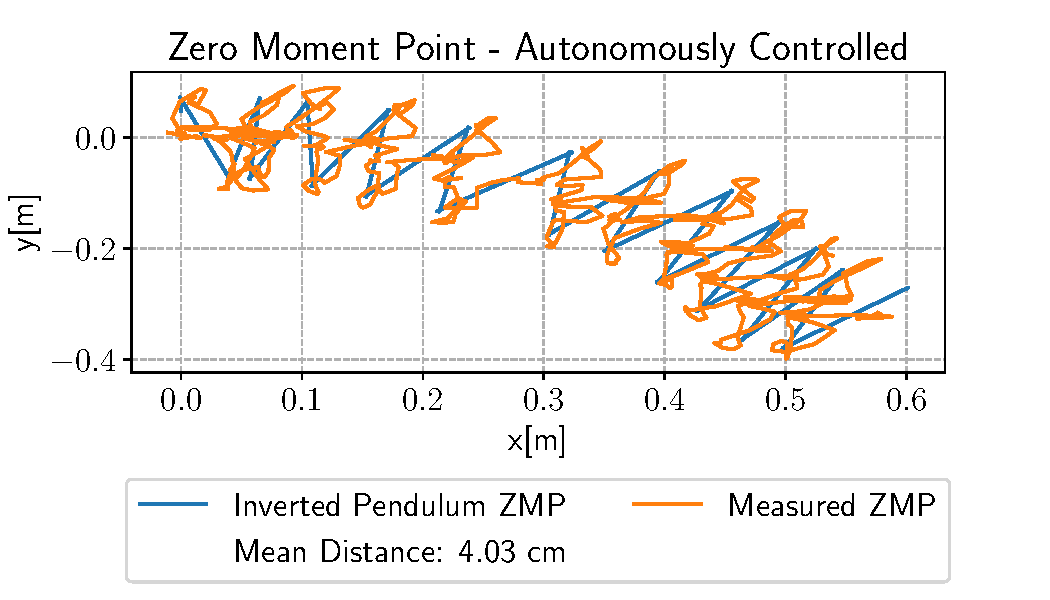
\includegraphics[scale=.45]{chapters/04_experiments/02_autonomous_walking/obstacle_walk_02_zmp.pdf}}
	\subcaptionbox{Behavior.}%
	[.5\linewidth]{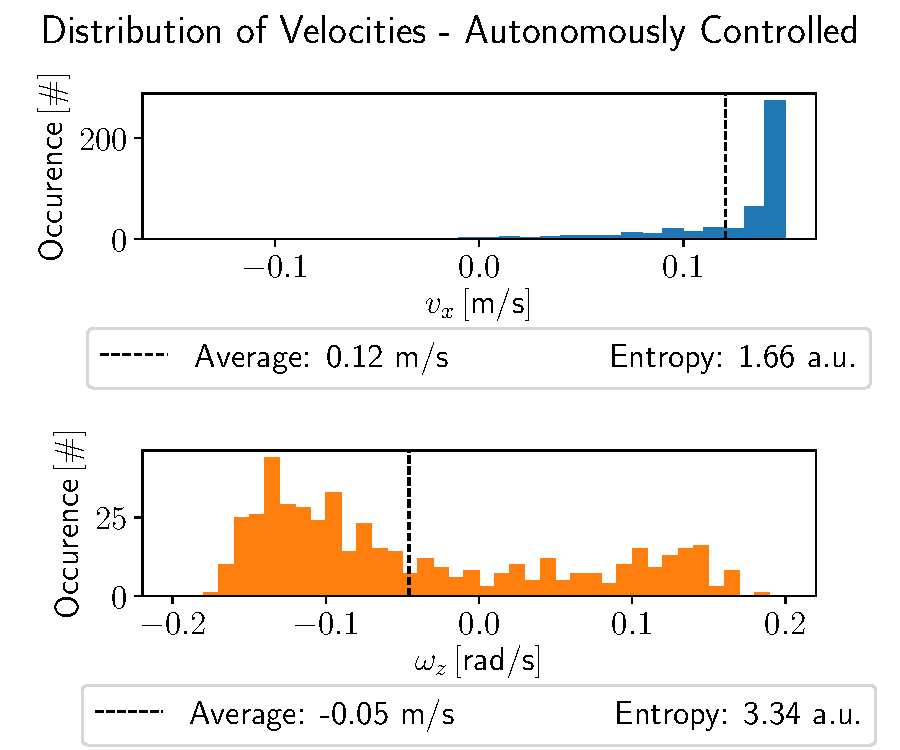
\includegraphics[scale=.45]{chapters/04_experiments/02_autonomous_walking/obstacle_walk_02_entropy.pdf}}
	\caption{Autonomously controlled obstacle avoidance. The robot started to the plot's left hand side (a), and avoided an obstacle by turning to the right, but then lost track of it.}
\label{fig::424_aw_basic_obstacle}
\end{figure}
\begin{figure}[h!] 
	\subcaptionbox{Dynamic balance.}%
	[.5\linewidth]{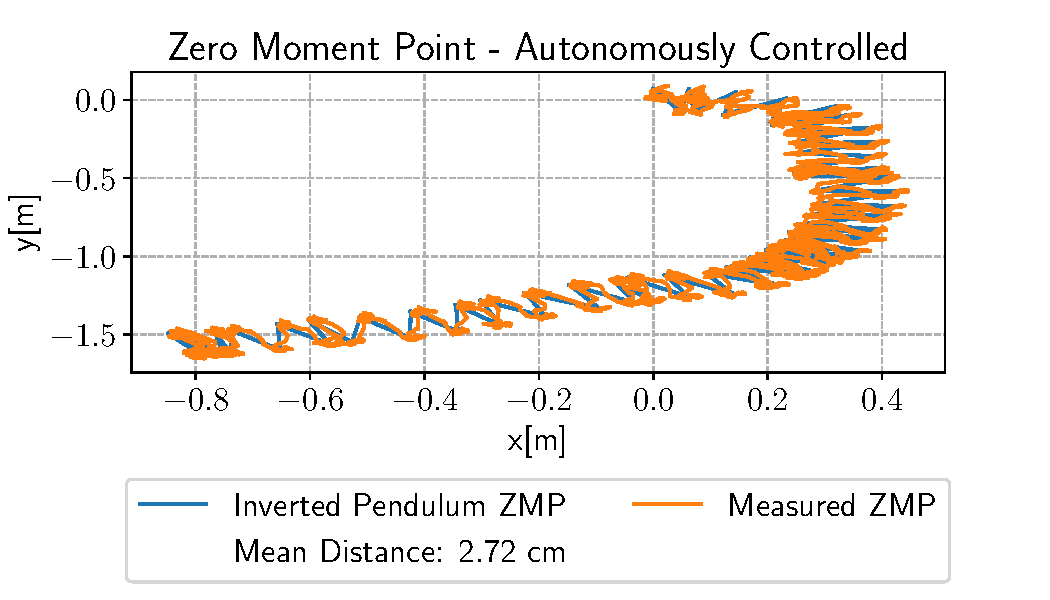
\includegraphics[scale=.45]{chapters/04_experiments/02_autonomous_walking/out_of_sight_walk_01_zmp.pdf}}
	\subcaptionbox{Behavior.}%
	[.5\linewidth]{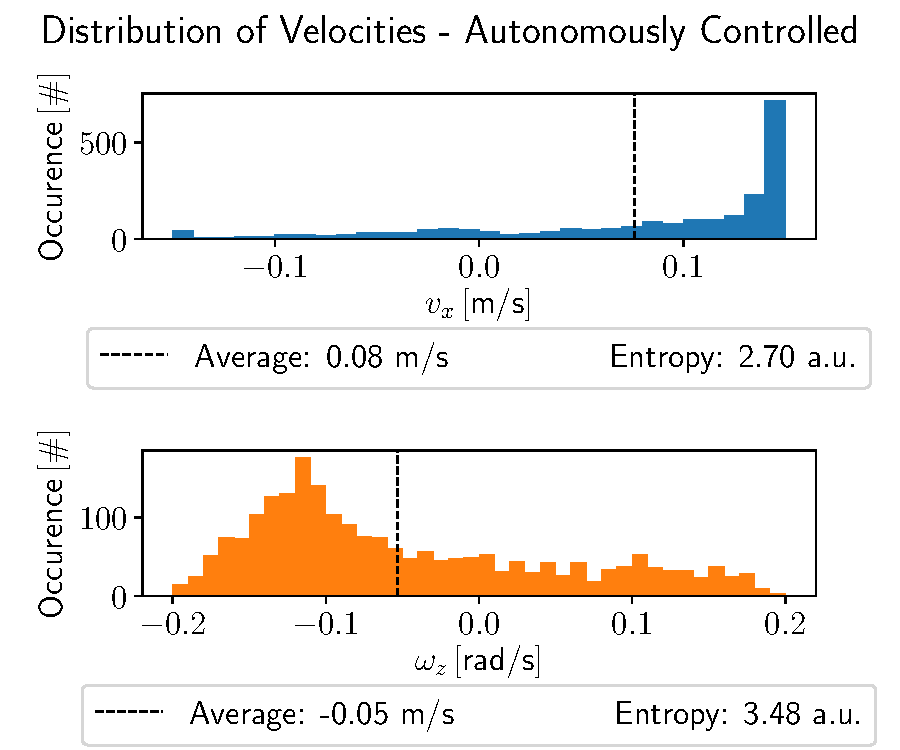
\includegraphics[scale=.45]{chapters/04_experiments/02_autonomous_walking/out_of_sight_walk_01_entropy.pdf}}
	\caption{Autonomously controlled environment scanning. The robot started to the plot's right hand side (a), facing to the right, and performed a turn to the right, until it saw the fire extinguisher and walked straight towards it.}
	\label{fig::424_aw_basic_sight}
\end{figure} 
In contrast to the validation split, there is no simple method anymore to compare the results of user controlled walking and autonomously controlled walking. This has two main reasons. First of all, a human, which controls the robot, does so from a third person perspective, while the neural network interacts with the environment from a first person perspective. Secondly, different actions that are taken, result in different states being in. That said, once the human agent and the artificial agent only take slightly different decisions, the two behaviors will be driven from completely different states, which causes yet another different action. We can therefore only compare whether or not the task of interest got solved, and how the different behaviors influenced the primal goal of dynamic balance, which brings us back to the observation of the neural network's noisy policy. To assess the level of noise, we computed the entropy $S(p(v))$ within the velocity distributions as follows
\begin{align}
	S(p(v)) = \sum_{v\in \bm{V}}p(v)\log p(v)
\end{align}
Furthermore, to rate the dynamic balance, we computed the mean distance of the inverted pendulum zero moment point from the pattern generator, and the measured zero moment point. We did so for every behavior and dynamic balance plot of our benchmarking setup. We then plotted the mean distance against the entropy in figure \ref{fig::424_entropy_balance}, in order to probe the influence of noisy decisions onto the balance.
\begin{figure}[h!]
	\centering
	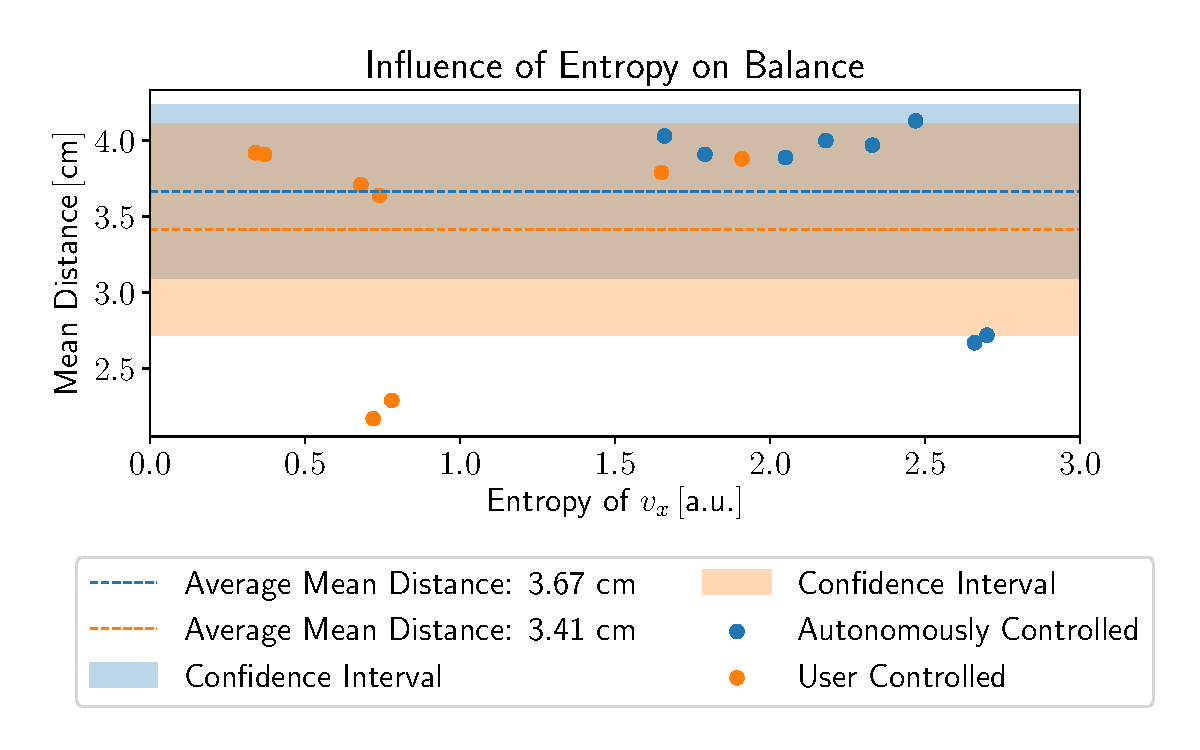
\includegraphics[scale=.5]{chapters/04_experiments/02_autonomous_walking/entropy_against_balance.pdf}
	\caption{Influence of entropic commands onto Heicub's dynamic balance. It can be seen that within the confidence interval there is no effect of the command signal's entropy on the robot's balance.}
	\label{fig::424_entropy_balance}
\end{figure}
The average mean distance with the standard deviation for user controlled walking therein is $3.41\pm0.69\,\text{cm}$, while that of autonomously controlled walking is $3.67\pm0.56\,\text{cm}$. Within the $1\sigma$-range, we could therefore demonstrate that the control signal's entropy does not have an affect on the balance. In addition to the benchmarking tasks, we further wanted to demonstrate the robot's behavior in two more scenarios. The first additional scenario involves a dynamic environment, in which the robot interacts with a human and a moving fire extinguisher. The second additional scenario simply demonstrates semantic understanding of the neural network, in that it poses the challenge of having similarly colored objects to distinguish from. Both additional tests are shown in figure \ref{fig::424_aw_gif_additional}, and they were solved successfully.
\begin{figure}[h!]
	\centering
	\subcaptionbox{Dynamic environment - \href{https://drive.google.com/file/d/1zm-9apobNmsXAcLXB5e9lGqIU7NMHzVl/view?usp=sharing}{\underline{link}}.}%
	[.4\linewidth]{\animategraphics[height=1.2in,loop,autoplay]{20}{chapters/04_experiments/02_autonomous_walking/dynamic_walk_01/frame-}{001}{031}}
	\subcaptionbox{Semantic understanding - \href{https://drive.google.com/file/d/1VQIEChA61GDxm-rLf8pfOxCgXeJhuFG9/view?usp=sharing}{\underline{link}}.}%
	[.4\linewidth]{\animategraphics[height=1.2in,loop,autoplay]{20}{chapters/04_experiments/02_autonomous_walking/semantic_walk_01/frame-}{001}{046}}
	\caption{Heicub's behavior in the test environment for additional tasks. The robot within these trials was controlled by the Unet model, shown in figure \ref{fig::423_unet}.}
\label{fig::424_aw_gif_additional}
\end{figure} 
Especially in the behavior plot of figure \ref{fig::424_aw_additional_semantic}, we can see that the robot successfully managed to walk backwards to avoid a collision with the human. Given the successful results of our first approach to train a neural network on autonomous navigation, we then continued to evaluate the proximal policy optimization algorithm, which got described in section \ref{sec::223_rl}.
\begin{figure}[h!]
	\subcaptionbox{Dynamic balance.}%
	[.5\linewidth]{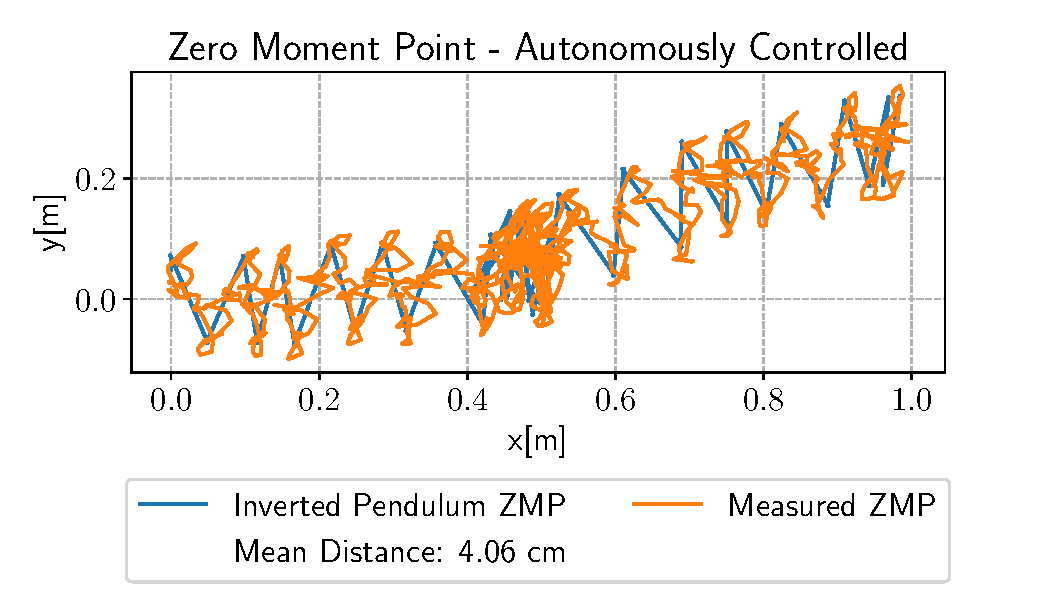
\includegraphics[scale=.45]{chapters/04_experiments/02_autonomous_walking/dynamic_walk_01_zmp.pdf}}
	\subcaptionbox{Behavior.}%
	[.5\linewidth]{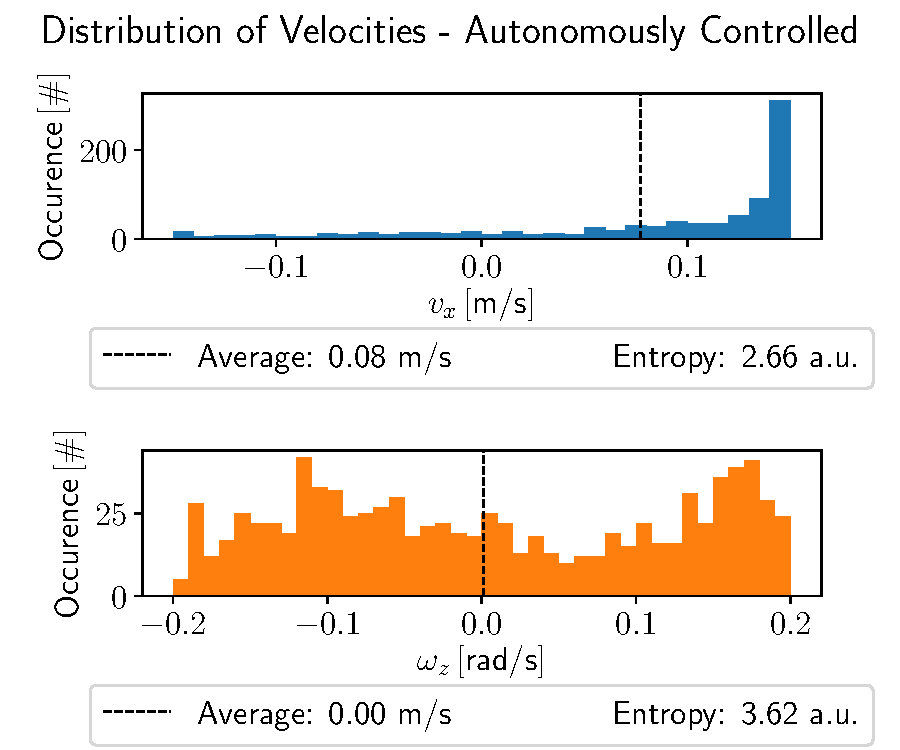
\includegraphics[scale=.45]{chapters/04_experiments/02_autonomous_walking/dynamic_walk_01_entropy.pdf}}
	\caption{Autonomously controlled in a dynamic environment. The robot started to the plot's left hand side, and moved forward towards the fire extinguisher, where it stopped on half way to avoid a human, until the pathway was free again.}
	\label{fig::424_aw_additional_dynamic}
\end{figure}
\begin{figure}[h!]
	\subcaptionbox{Dynamic balance.}%
	[.5\linewidth]{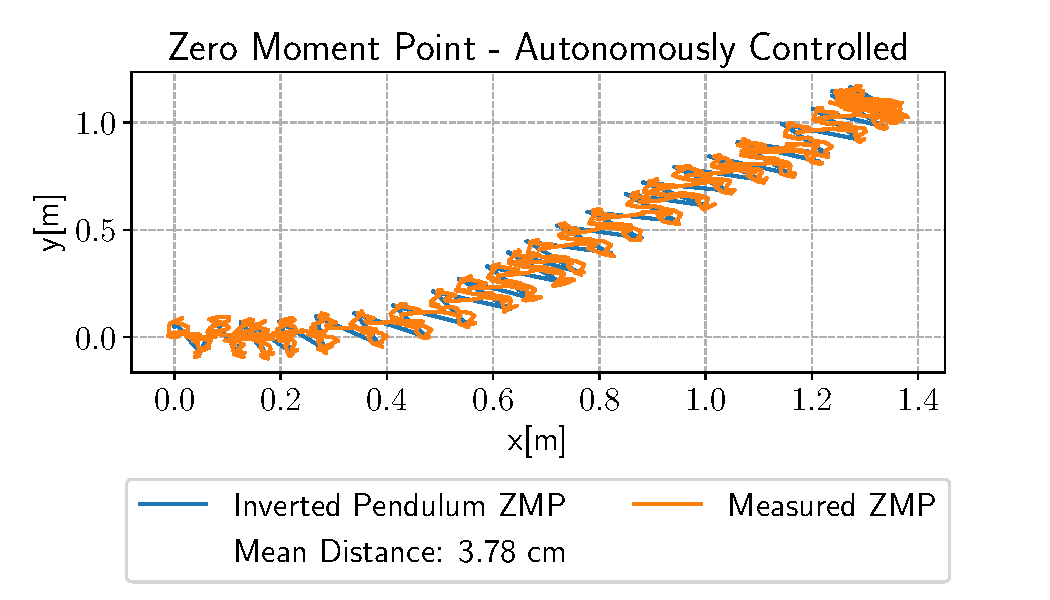
\includegraphics[scale=.45]{chapters/04_experiments/02_autonomous_walking/semantic_walk_01_zmp.pdf}}
	\subcaptionbox{Behavior.}%
	[.5\linewidth]{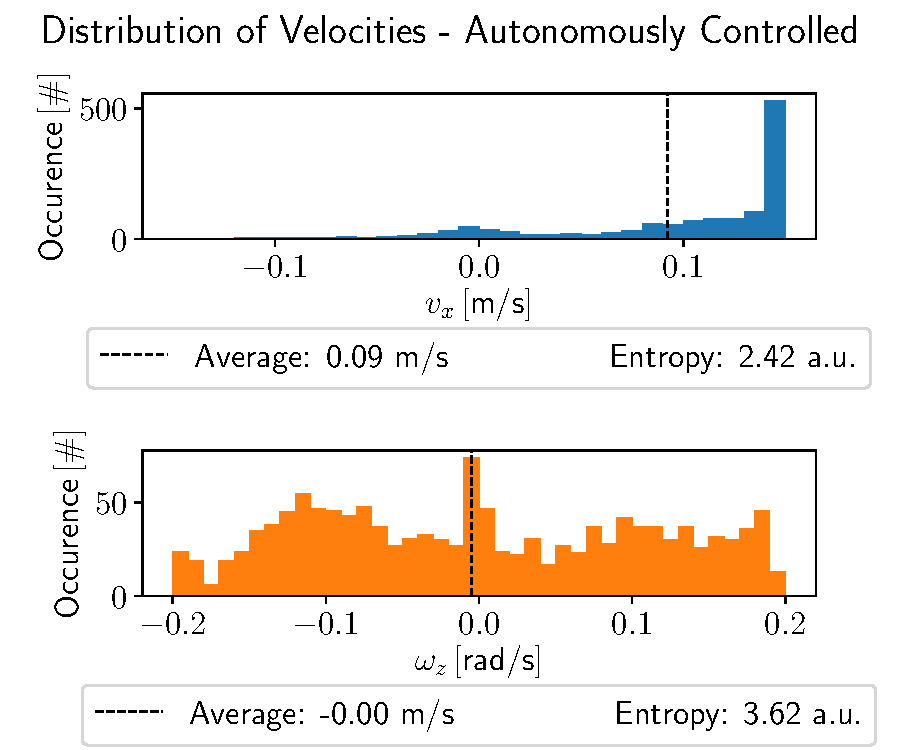
\includegraphics[scale=.45]{chapters/04_experiments/02_autonomous_walking/semantic_walk_01_entropy.pdf}}
	\caption{Autonomously controlled for demonstration of semantic understanding. The robot started to the plot's left hand side (a), and moved forward to the fire extinguisher to its left. Heicub had to distinguish between the fire extinguisher and another orange object right in front of it.}
	\label{fig::424_aw_additional_semantic}
\end{figure}
\subsection{Proximal Policy Optimization}
\label{sec::425_pp}
Since there is to this date no feasible way of training an agent on autonomous navigation in real time with reinforcement learning, we decided to implement a benchmarking environment that is shown in figure \ref{fig::425_ppo_env}. The agent's goal within this setup is to move towards the red dot, while keeping a maximum distance of $10\,\text{a.u.}$ towards it. The environment's state is simply described by a concatenation of the agent's position $\bm{a} = \begin{pmatrix}
a_x & a_y
\end{pmatrix}^T$ with that of the goal $\bm{g} = \begin{pmatrix}
g_x & g_y
\end{pmatrix}^T$. The reward $r_t$, at time step $t$, is designed to encourage motion towards the goal, by taking the difference of the previous and the current goal distance $r_t = ||\bm{a}_{t-1}-\bm{g}_{t-1}||_2 - ||\bm{a}_{t}-\bm{g}_{t}||_2$. Furthermore, a reward of ten was gained for successful completion, while a reward of negative ten was granted for whenever the agent left the maximally allowed distance towards the goal, see for example figure \ref{fig::425_ppo_env} (a).
\begin{figure}[h!]
	\centering
	\subcaptionbox{Agent at epoch 1.}%
	[.45\linewidth]{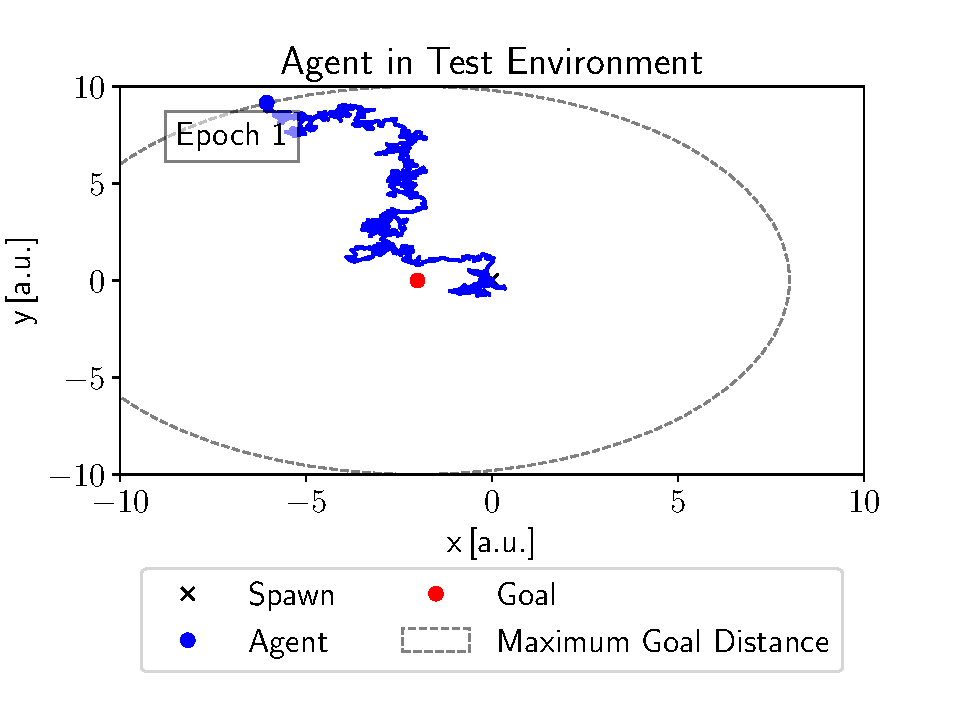
\includegraphics[scale=.45]{chapters/04_experiments/02_autonomous_walking/epoch_1.pdf}}	
	\subcaptionbox{Agent at epoch 30.}%
	[.45\linewidth]{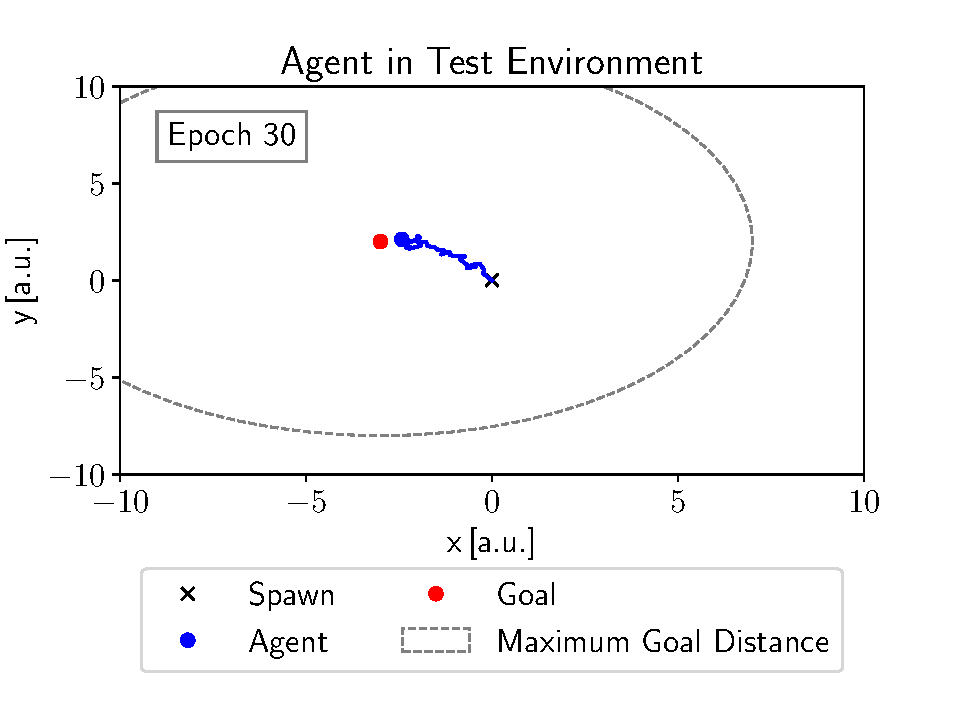
\includegraphics[scale=.45]{chapters/04_experiments/02_autonomous_walking/epoch_30.pdf}}
	\caption{Artificial agent in proximal policy optimization test environment. It can be seen that while the agent acts randomly in epoch 1 (a), the goal is reached with high confidence at epoch 30 (b).}	
	\label{fig::425_ppo_env}
\end{figure} 
In each of the cases, the environment was reset, and the goal got spawned at a random location. For both, the agent and the critic network, we used a fully connected neural network with 2 hidden layers of size 16, and 32, respectively. The output layer provided 2 units, which reflect our agent's degrees of freedom in the environment. For the hidden units, we again relied on rectifying linear units as our activation function, while we used a hyperbolic tangent for the output. We were able to produce the best results with a gradient clipping at $\epsilon=0.2$ (see equation \ref{eq::223_clip}), and the cost function hyper-parameters $c_1 = 0.5$ and $c_2 = 0.1/\overline{r_t}$, where $\overline{r_t}$ denotes the average reward, and which can be found in equation \ref{eq::223_ppo_loss}. 
\begin{figure}[h!]
	\centering
	\subcaptionbox{Reward history.}%
	[.45\linewidth]{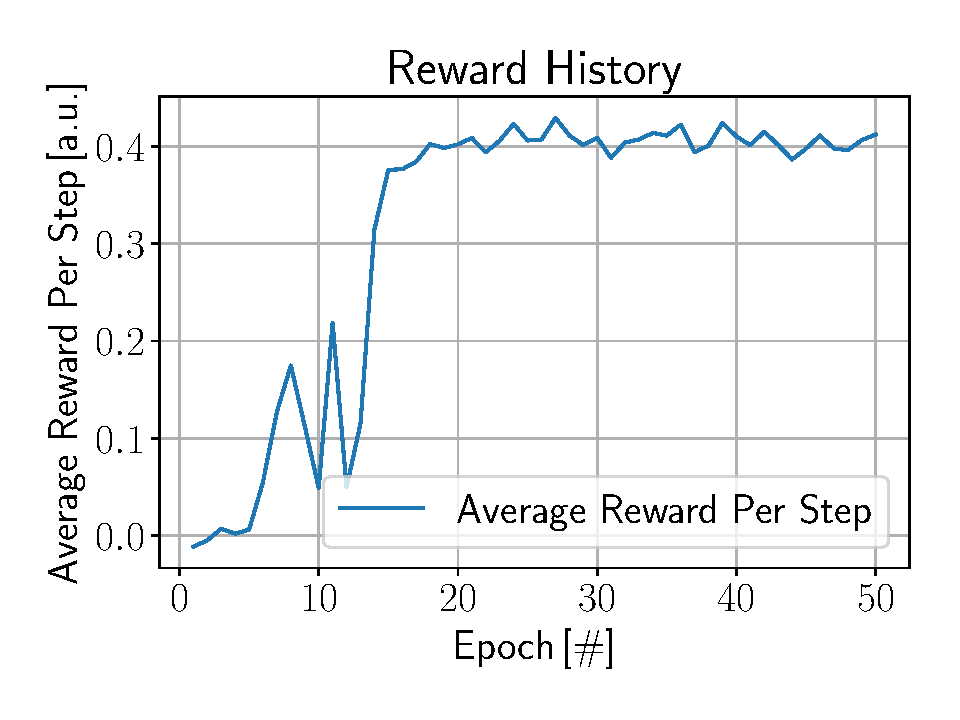
\includegraphics[scale=.35]{chapters/04_experiments/02_autonomous_walking/ppo_reward_history.pdf}}	
	\subcaptionbox{Standard deviation history.}%
	[.45\linewidth]{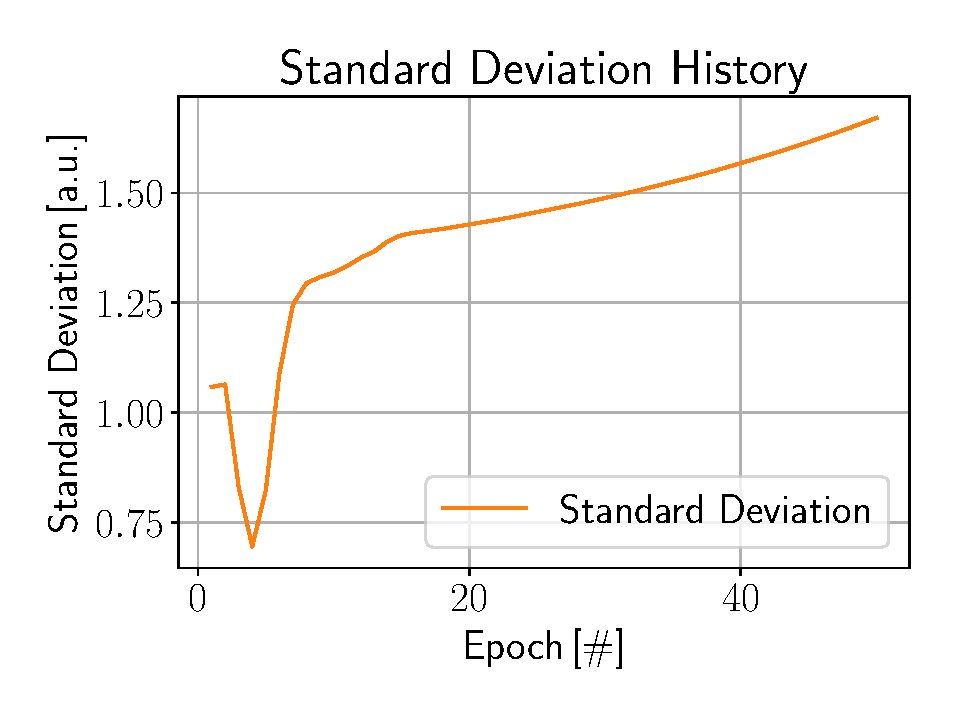
\includegraphics[scale=.35]{chapters/04_experiments/02_autonomous_walking/ppo_std_history.pdf}}
	\caption{Proximal policy optimization in test environment over 50 epochs. The agent learned to maximize the reward after around 20 epochs, by increasing its exploration with a higher standard deviation within the policy $\pi_\theta$ (b).}	
	\label{fig::425_ppo_hist}
\end{figure}
We ran the environment for $10000$ steps per epoch, and updated the networks every $4096$ actions, with a minibatch size of $M=512$ for $8$ proximal policy optimization epochs (see algorithm \ref{alg::225_ac}). The Adam optimizer then led to convergence at a learning rate of $0.01$ after about thirty epochs (see figure \ref{fig::425_ppo_hist}). A main reason for the fast convergence was caused by the chosen entropy hyperparameter $c_2$, which encouraged exploration on low rewards, and damped exploration on high rewards. We computed the entropy $S[\pi_\theta]$ from the differential entropy of our Gaussian policy $\pi_\theta$ via (\href{https://github.com/mhubii/ppo_libtorch/blob/481c1e326dcd6220b2c1c955a0303a410c2cb0dd/Models.h#L82}{\underline{link}})
\begin{align}
	S[\pi_\theta] = 0.5 + 0.5\log(2\pi)+\log(\sigma),
\end{align}
where $\sigma$ is the standard deviation. We can then see the standard deviation's influence on the reward, as it starts to increase strongly in figure \ref{fig::425_ppo_hist} (b). After having trained the agent successfully for $50$ epochs, we ran the policy $\pi_\theta$ without noise contribution, but rather took the average $\mu$, as proposed by the actor network. An example of the agent's behavior can be seen in figure \ref{fig::425_ppo_test}, which now appears really smooth. 
\begin{figure}[h!]
	\centering
	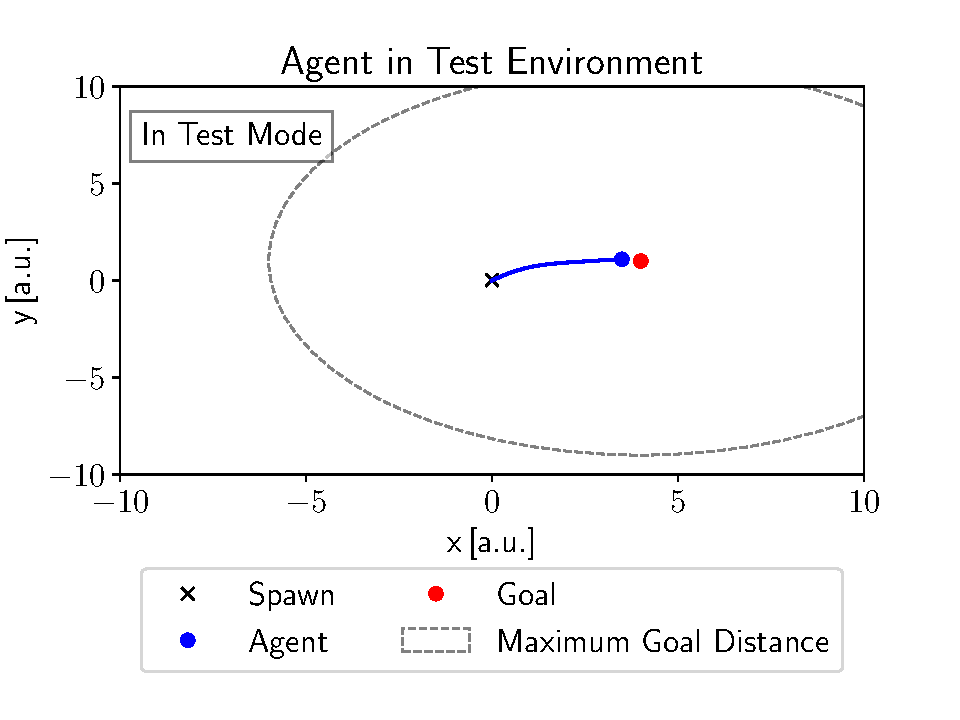
\includegraphics[scale=.45]{chapters/04_experiments/02_autonomous_walking/test_mode.pdf}
	\caption{Proximal policy optimization in test mode, that is without noisy policy $\pi_\theta$. It can be seen that the agent almost learned to move the shortest path towards the goal.}	
	\label{fig::425_ppo_test}
\end{figure}
We ran the agent ten times for $10000$ steps without noise contribution, and observed $311\pm3$ wins on average, and no lost game at all, which indicates that the neural network learned to generalize the task well.